\documentclass{article}

\usepackage{graphicx}
\usepackage{amsmath}
\usepackage{amssymb}
\usepackage{booktabs}
\usepackage{hyperref}

\title{Weight-Space Symmetry in Low-Rank Networks}
\author{Anonymous Author(s)}

\begin{document}

\maketitle

\begin{abstract}
We study how low-rank neural networks learn even one-dimensional targets and how the learned symmetry appears in their internal partial functions and in weight space. Starting from MMNN/RF-LR experiments on $y(x)=\sum_{k=1}^{3}\cos(2\pi kx)$, we compare low-rank bottleneck partials with full-rank MLP hidden features. The central hypothesis is that MMNN/RF-LR models preserve target symmetry through mirrored random-feature atoms and matched outgoing coefficients, while full-rank networks can reach low loss through asymmetric hidden representations. We connect this to the plateau-sharp-plateau training dynamics observed around learning-rate reductions.
\end{abstract}

\section{Motivation}

The ICLR landscape experiments show that learning-rate reductions coincide with sharp loss drops and visible changes in partial functions. In the $f_3$, $N=768$, batch-size $8$, depth $L=3$ setting, partial functions before and after LR divides suggest that internal representation geometry changes when the trajectory enters a sharper valley. This workshop paper focuses on the symmetry aspect of that phenomenon.

\section{Setup}

The target is even:
\[
y(x)=\sum_{k=1}^{3}\cos(2\pi kx), \qquad x\in[-1,1].
\]
We compare MMNN/RF-LR models with frozen rank-to-width feature maps against full-rank MLPs trained on the same grid and optimizer schedule. For a learned function $g$, the output symmetry defect is
\[
D_{\mathrm{out}}=\frac{\mathbb{E}_{x>0}\left[(g(x)-g(-x))^2\right]}{\mathbb{E}_{x>0}\left[g(x)^2\right]}.
\]
The same quantity is computed for layerwise partial functions.

\section{Weight-Space Mirror Metric}

For first-layer ReLU atoms of the form $\mathrm{ReLU}(a_jx+b_j)$, an even representation can be built from mirror pairs $(a_j,b_j)$ and $(-a_j,b_j)$ with matched outgoing coefficients. We therefore measure, for each atom, the nearest mirror atom and the relative outgoing coefficient mismatch. Low mismatch among close mirror pairs is evidence that symmetry is encoded directly in weight space.

\section{Current Figures}

The first automatic diagnostic run used two seeds, width $256$, rank $10$, depth $3$, $N=384$, batch size $8$, and $600$ epochs. Both architectures learn nearly even outputs, but their internal representations differ: the final MMNN bottleneck has symmetry defects $3.28\cdot 10^{-3}$ and $5.76\cdot 10^{-3}$ across the two seeds, while the final MLP hidden layer has defects $1.26$ and $1.37$. This supports the intended distinction between output symmetry and partial-function symmetry.

A longer grid then trained $16$ configurations for $2000$ epochs each: seeds $42,43$, width $384$, depths $2,3$, MMNN ranks $5,10,20$, plus matched full-rank MLPs. Because some MLP channels have nearly zero energy, we report active-channel partial defects by filtering channels above median energy in each layer. The result is stable: MLP outputs can be nearly even, but their active hidden partials remain asymmetric; MMNN depth-$3$ late bottleneck partials are often close to even.

\begin{figure}[h]
\centering
\includegraphics[width=0.88\linewidth,height=0.72\textheight,keepaspectratio]{../../experiments/table/results_sumcos_selected_rerun/f3_N768_bs8_L3/plot_partial_before_after_lr_divides.png}
\caption{Partial functions before and after LR divides for $f_3$, $N=768$, batch size $8$, depth $L=3$. This is the current source image behind the ICLR Figure 5 claim.}
\end{figure}

\begin{figure}[h]
\centering
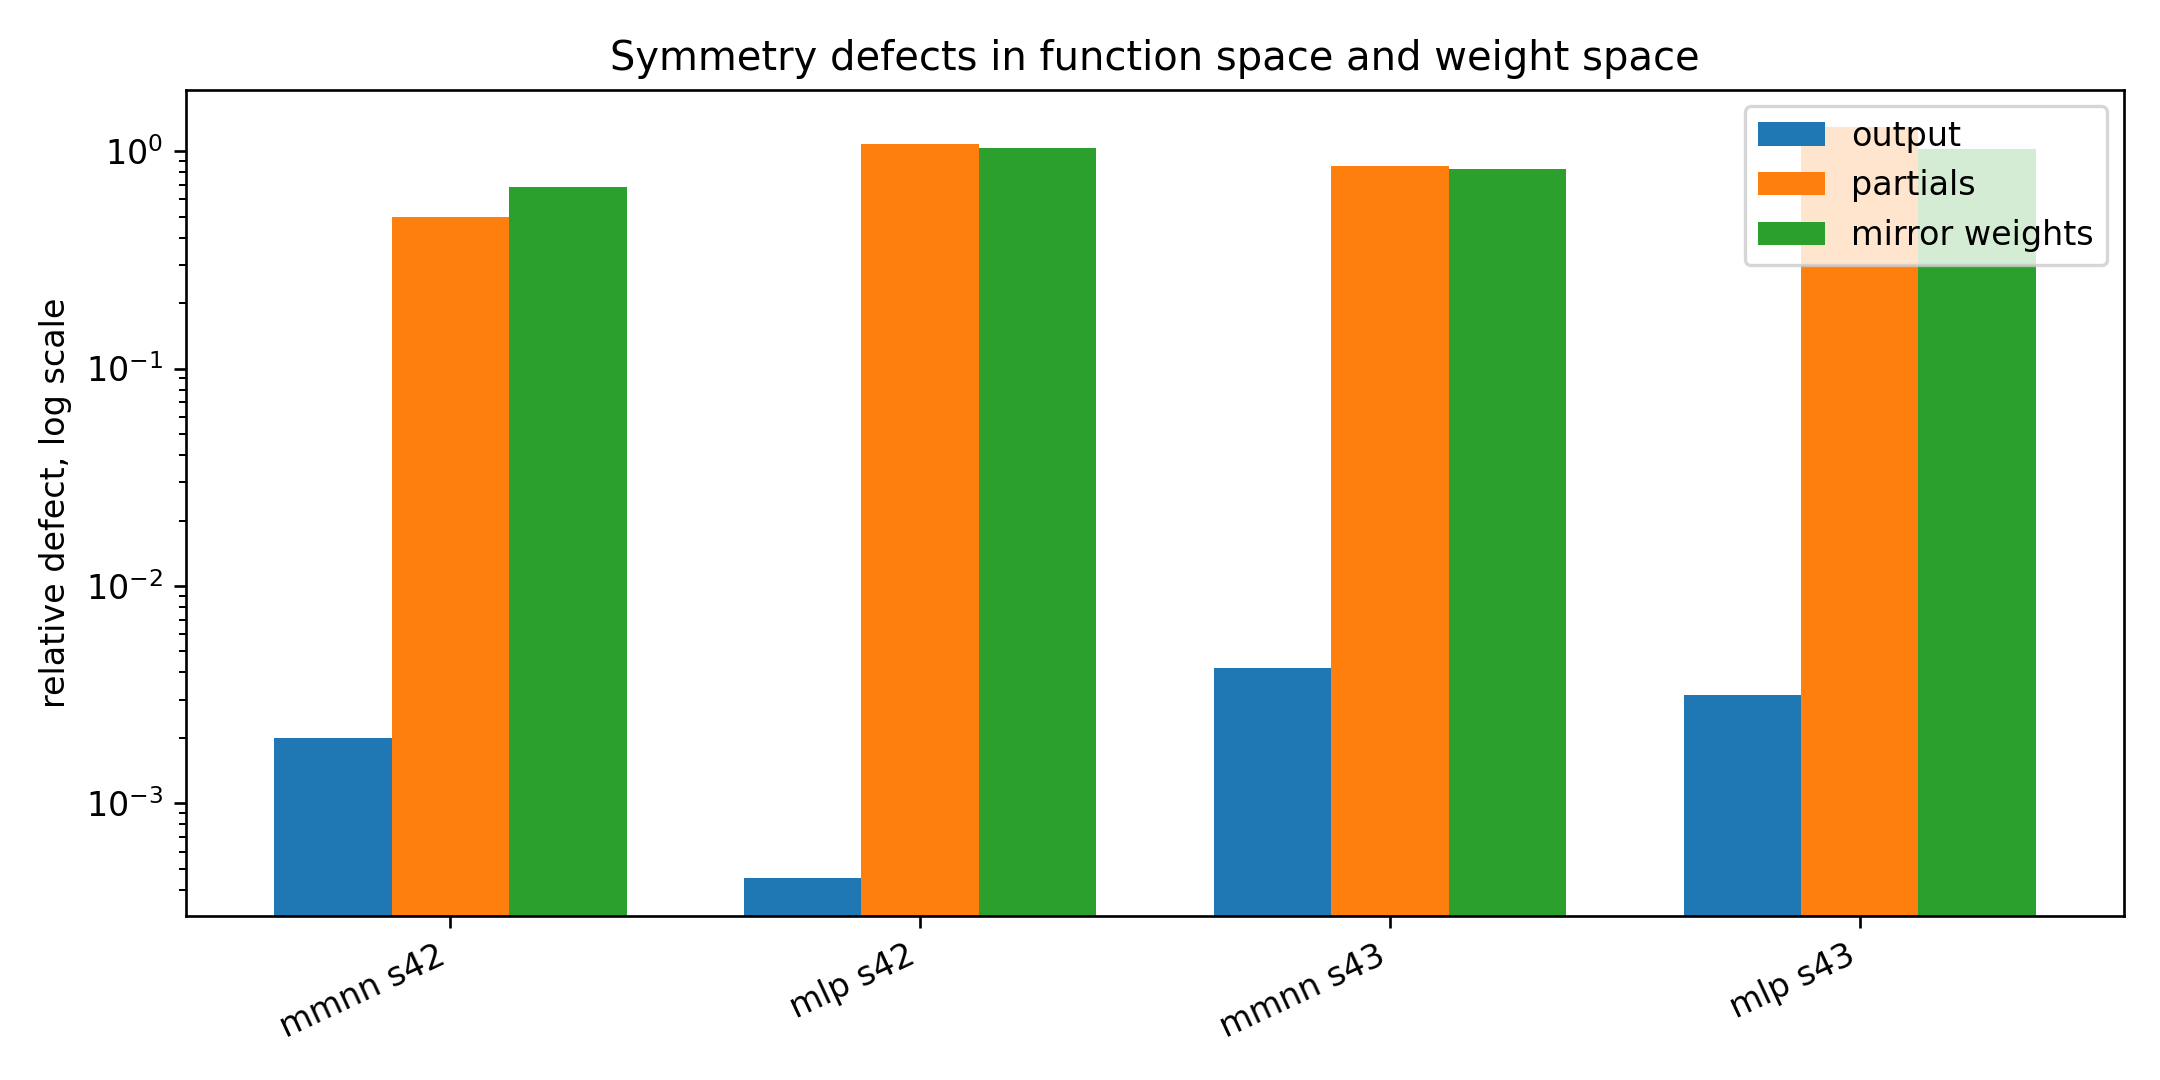
\includegraphics[width=0.72\linewidth]{results/symmetry_weightspace/symmetry_defects_bar.png}
\caption{Automatic quick-run diagnostic: output, partial-function, and mirror-pair weight-space symmetry defects.}
\end{figure}

\begin{figure}[h]
\centering
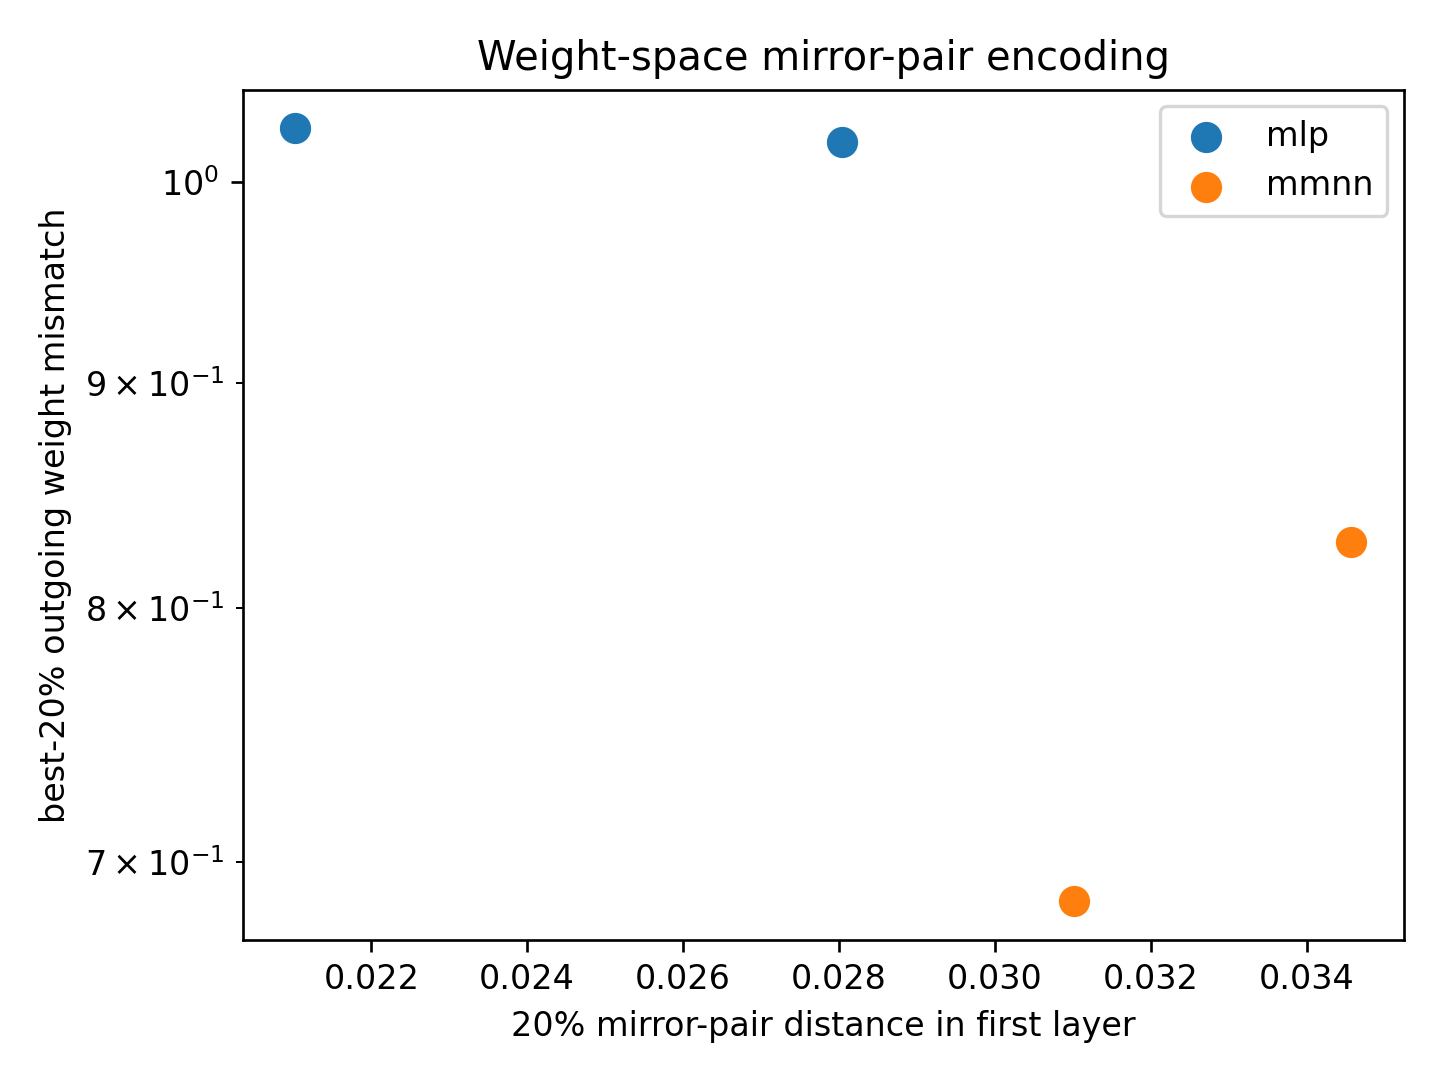
\includegraphics[width=0.72\linewidth]{results/symmetry_weightspace/mirror_pair_weightspace.png}
\caption{Mirror-pair weight-space diagnostic in the first layer.}
\end{figure}

\begin{figure}[h]
\centering
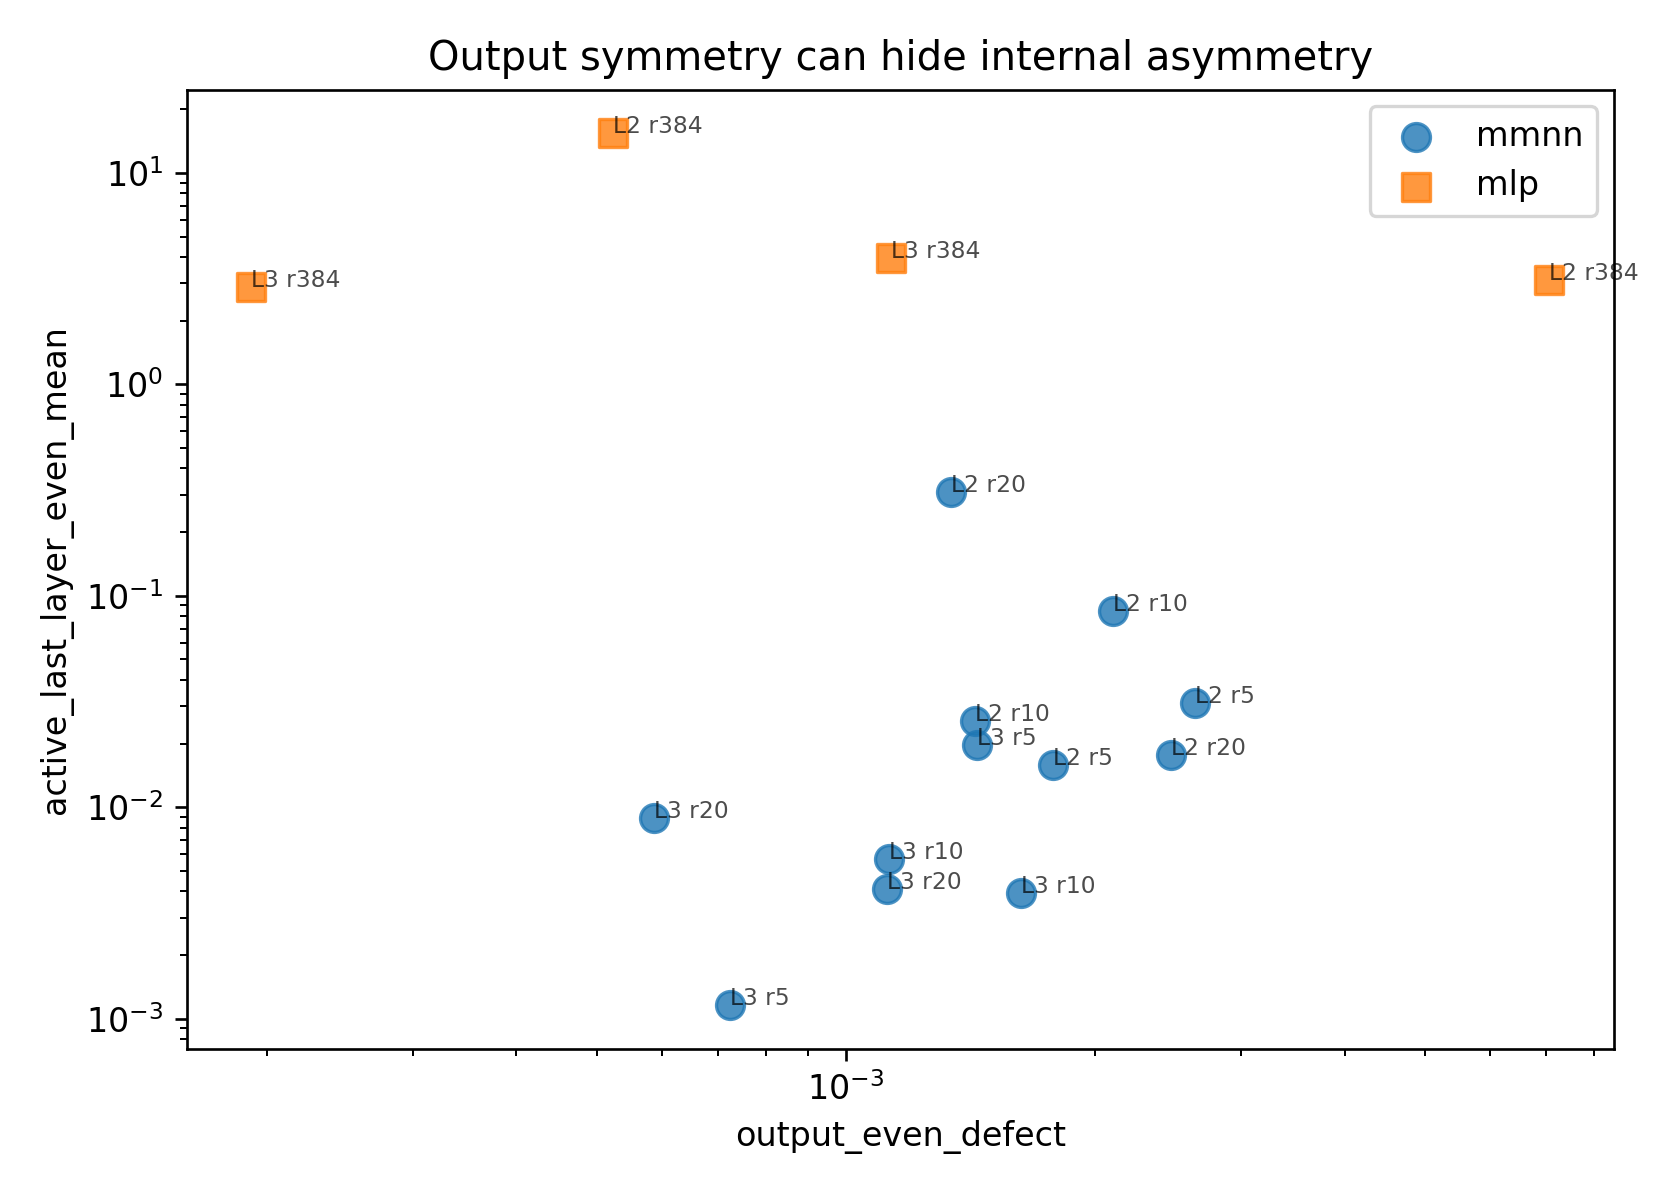
\includegraphics[width=0.72\linewidth]{results/symmetry_grid_long/active_output_vs_partial_symmetry.png}
\caption{Long-grid diagnostic: output-space symmetry versus active last-layer partial-function symmetry. Full-rank MLPs can have even outputs while keeping asymmetric active hidden features.}
\end{figure}

\begin{figure}[h]
\centering
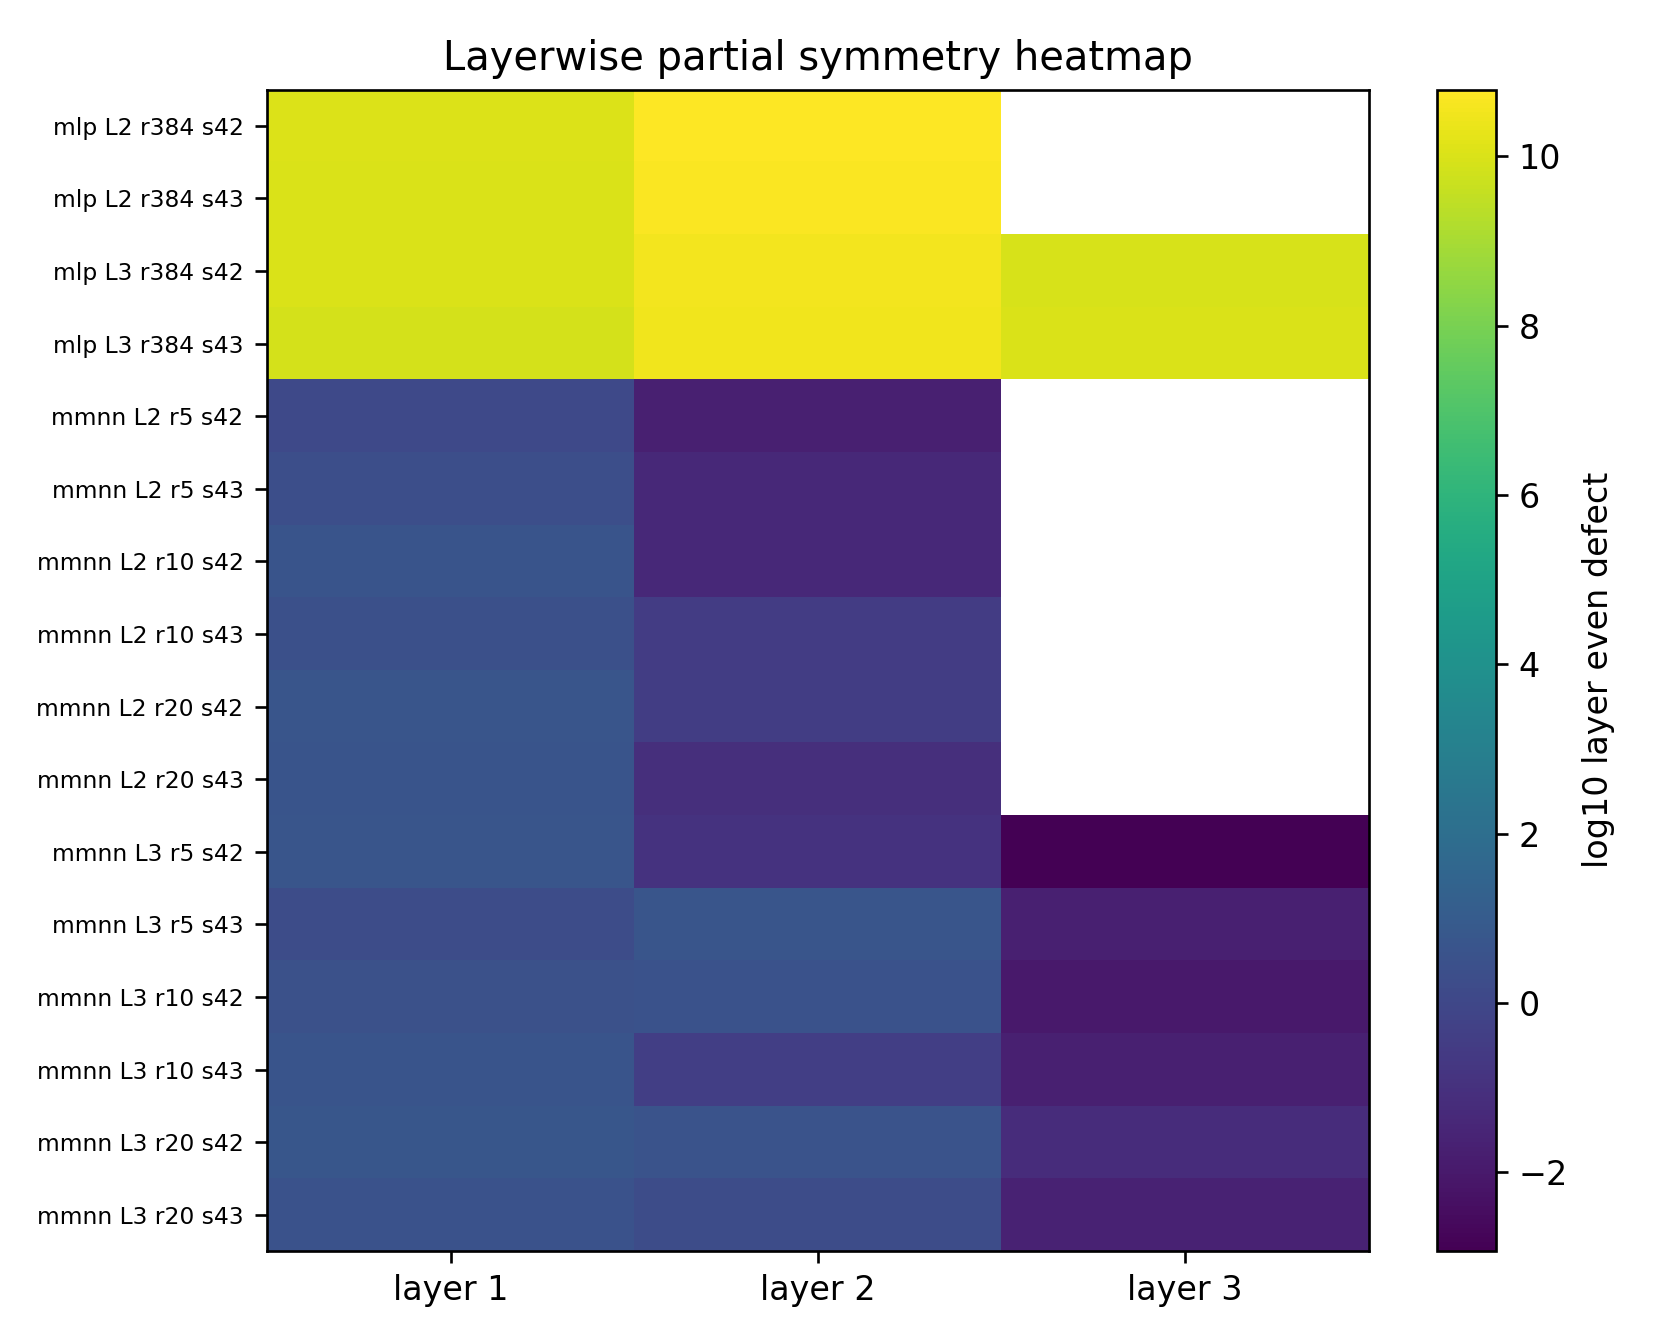
\includegraphics[width=0.72\linewidth]{results/symmetry_grid_long/layerwise_partial_symmetry_heatmap.png}
\caption{Layerwise partial-function symmetry heatmap across the long grid. The late MMNN bottleneck layers, especially at depth $3$, show much smaller active symmetry defects.}
\end{figure}

\begin{figure}[h]
\centering
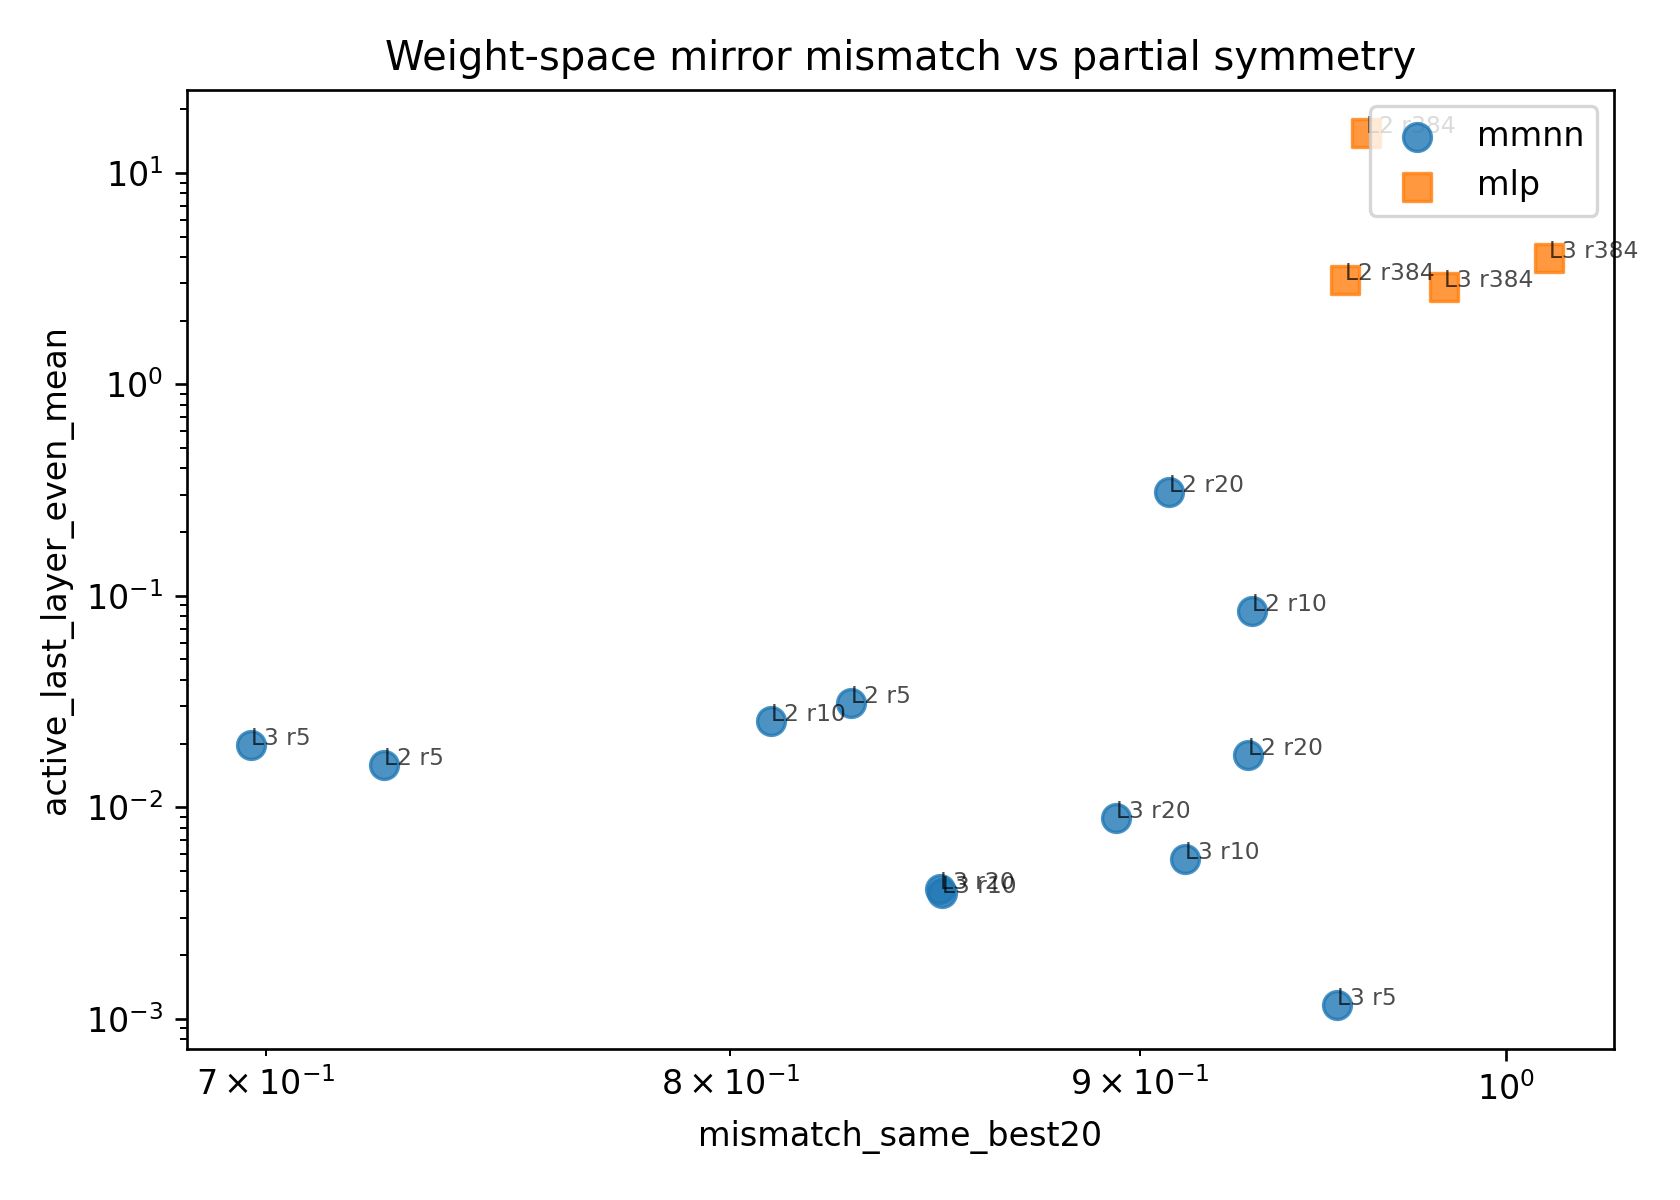
\includegraphics[width=0.72\linewidth]{results/symmetry_grid_long/active_weightspace_vs_partial_symmetry.png}
\caption{Weight-space mirror mismatch versus active partial symmetry. The current nearest-mirror metric moves in the expected direction but is weaker than the function-space separation.}
\end{figure}

\section{Low-Loss ICLR Configurations}

The strongest evidence comes from rerunning the actual low-loss sumcos configurations listed in the ICLR draft and baseline tables. These runs use the original MMNN setup with width $1024$, adaptive SGD, and factor-dependent grids. Unlike the MNIST ablations, these configurations reach test MSEs between $1.94\cdot 10^{-5}$ and $3.26\cdot 10^{-3}$. In this low-loss regime, the even-target symmetry is visible not only in the output but also in the late bottleneck partial functions.

Across six rerun configurations, output even defects range from $4.1\cdot 10^{-6}$ to $8.0\cdot 10^{-4}$, and active last-layer partial even defects range from $6.24\cdot 10^{-5}$ to $5.22\cdot 10^{-4}$. This is the cleanest current support for the central claim: when MMNNs truly learn the even sumcos target, the low-rank partial functions become strongly even. The nearest-mirror weight-space statistic also moves in the expected direction, with best-$20\%$ mirror-pair mismatch around $0.56$--$0.71$, but this remains weaker evidence than the function-space partials.

\begin{figure}[h]
\centering
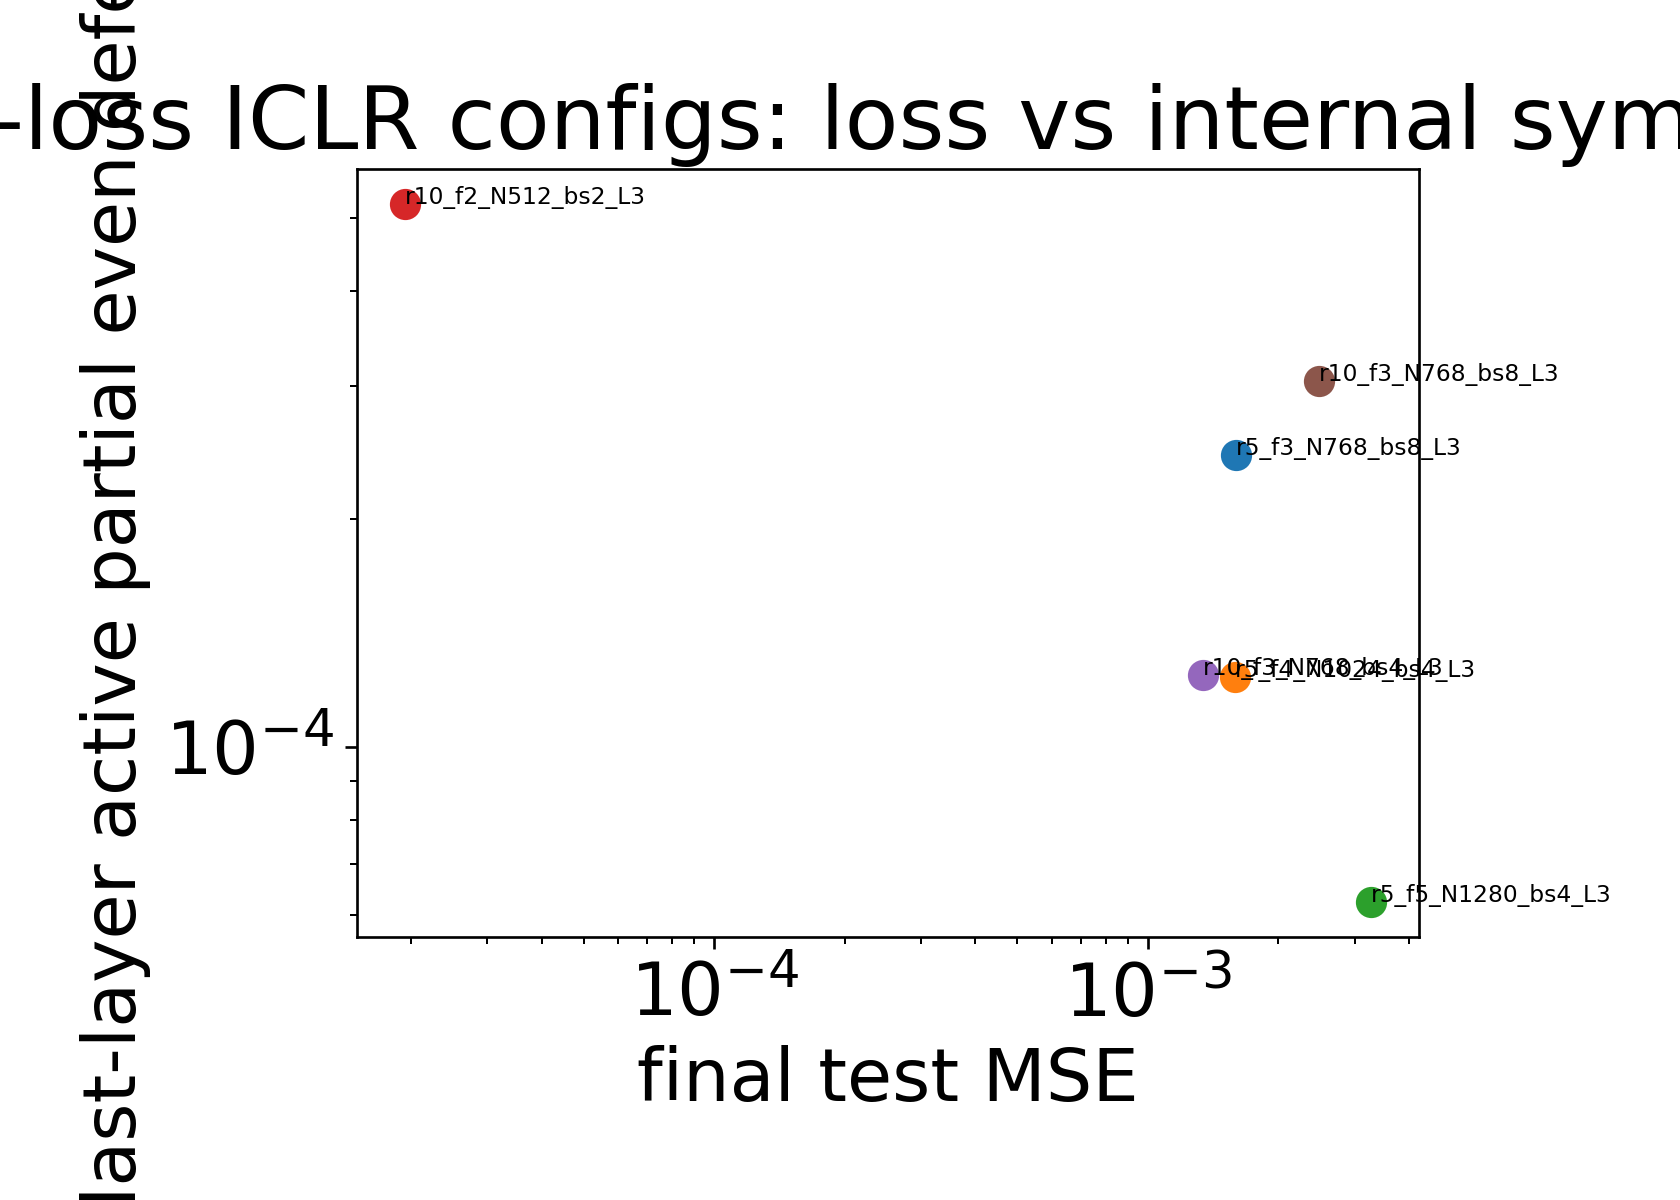
\includegraphics[width=0.72\linewidth]{results/good_sumcos_low_loss/low_loss_test_error_vs_partial_symmetry.png}
\caption{Low-loss ICLR configs: final test MSE versus active last-layer partial symmetry defect. These are the reliable symmetry runs.}
\end{figure}

\begin{figure}[h]
\centering
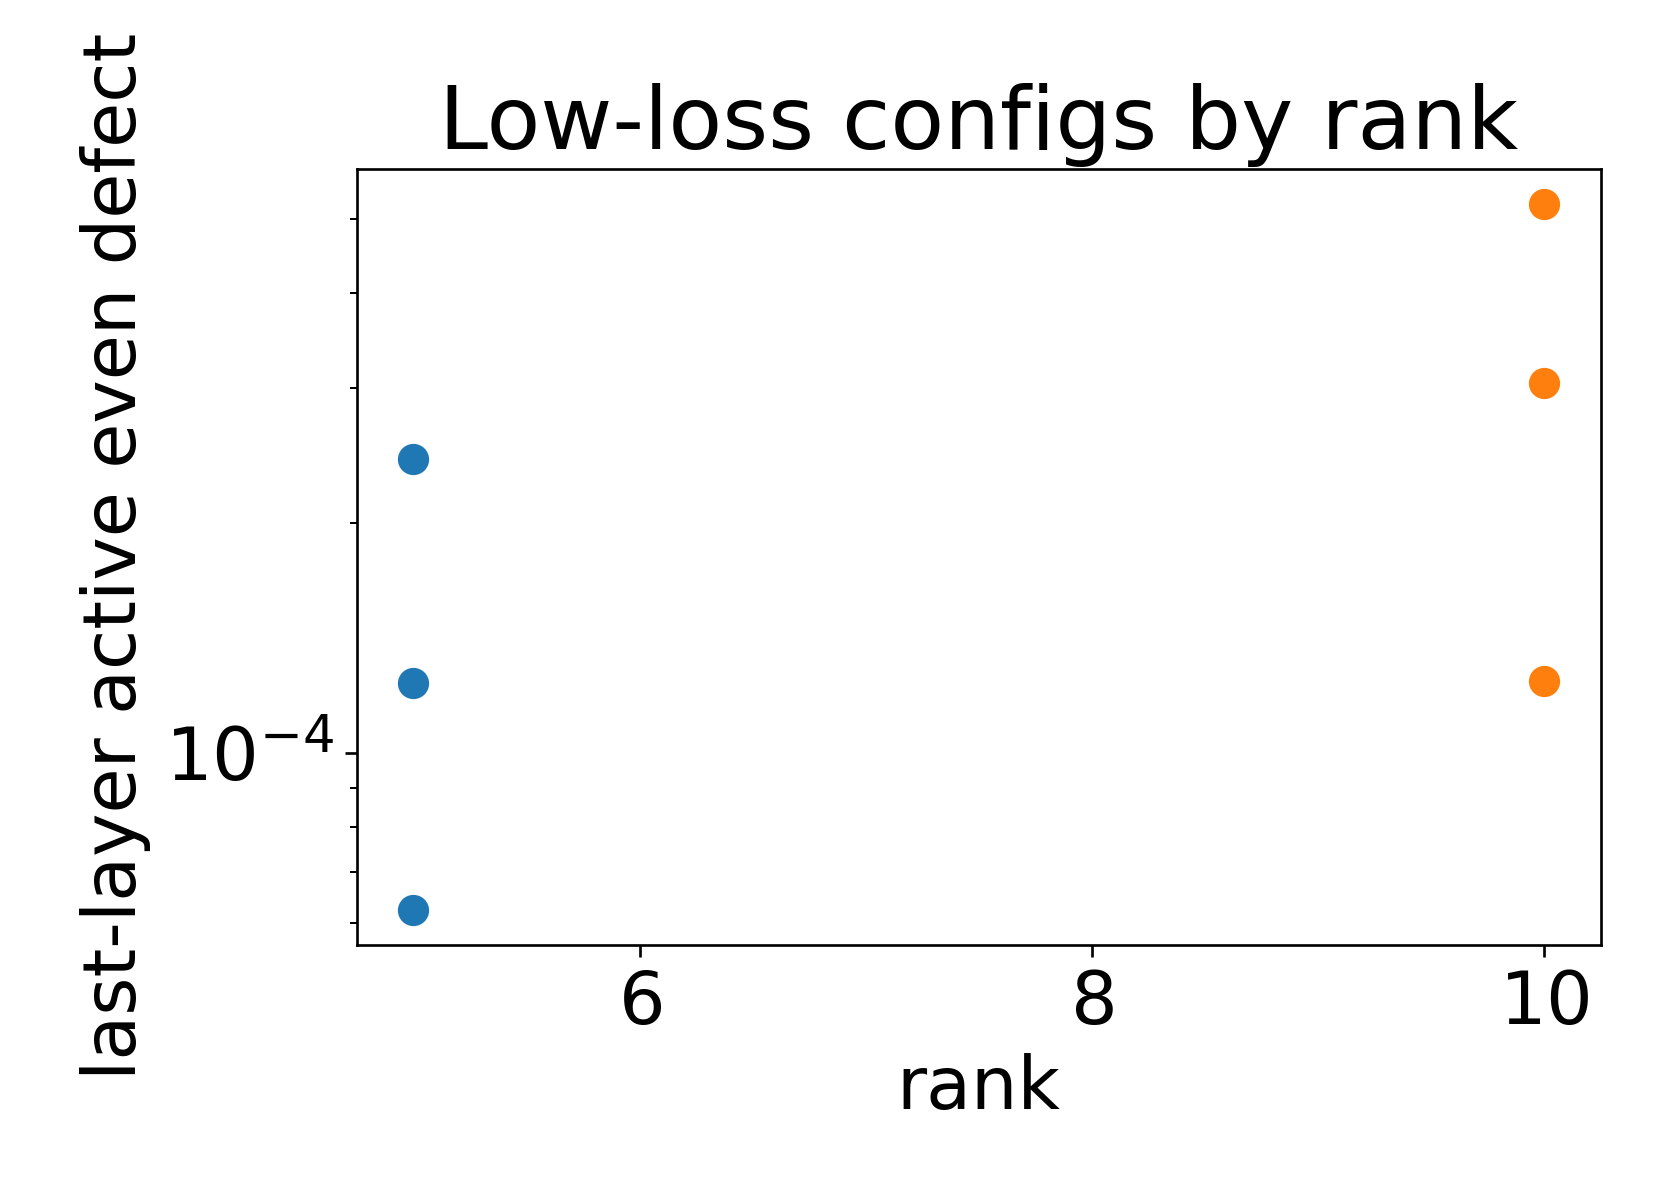
\includegraphics[width=0.72\linewidth]{results/good_sumcos_low_loss/low_loss_rank_vs_partial_symmetry.png}
\caption{Low-loss ICLR configs grouped by rank. Late bottleneck partials remain strongly even after fitting the target.}
\end{figure}

\section{Weight-Space Cases}

The exhaustive rerun gives a useful separation between output-space symmetry and internal symmetry. We classify completed checkpoints into three regimes: \emph{partial-symmetric} runs have low test MSE and active last-layer partial defect below $10^{-3}$; \emph{output-only/asymmetric} runs have low test MSE but active partial defect above $10^{-2}$; underfit runs have high test MSE. In the currently completed rerun, this yields $12$ partial-symmetric runs, $28$ output-only/asymmetric runs, $92$ intermediate runs, and $9$ underfit runs.

The most useful contrast is between two low-loss examples. A rank-$5$, $f_2$, $N=512$, batch-size-$1$, depth-$3$ run has test MSE $9.53\cdot 10^{-4}$ and active last-layer partial defect $2.62\cdot 10^{-5}$, making it a clean internally symmetric case. A rank-$10$, $f_1$, $N=256$, batch-size-$2$, depth-$1$ run has test MSE $1.17\cdot 10^{-4}$ but active partial defect $2.17$, showing that fitting an even target can still leave strongly asymmetric internal partials. This counterexample is important: it makes the positive MMNN symmetry claim nontrivial rather than tautological.

\begin{figure}[h]
\centering
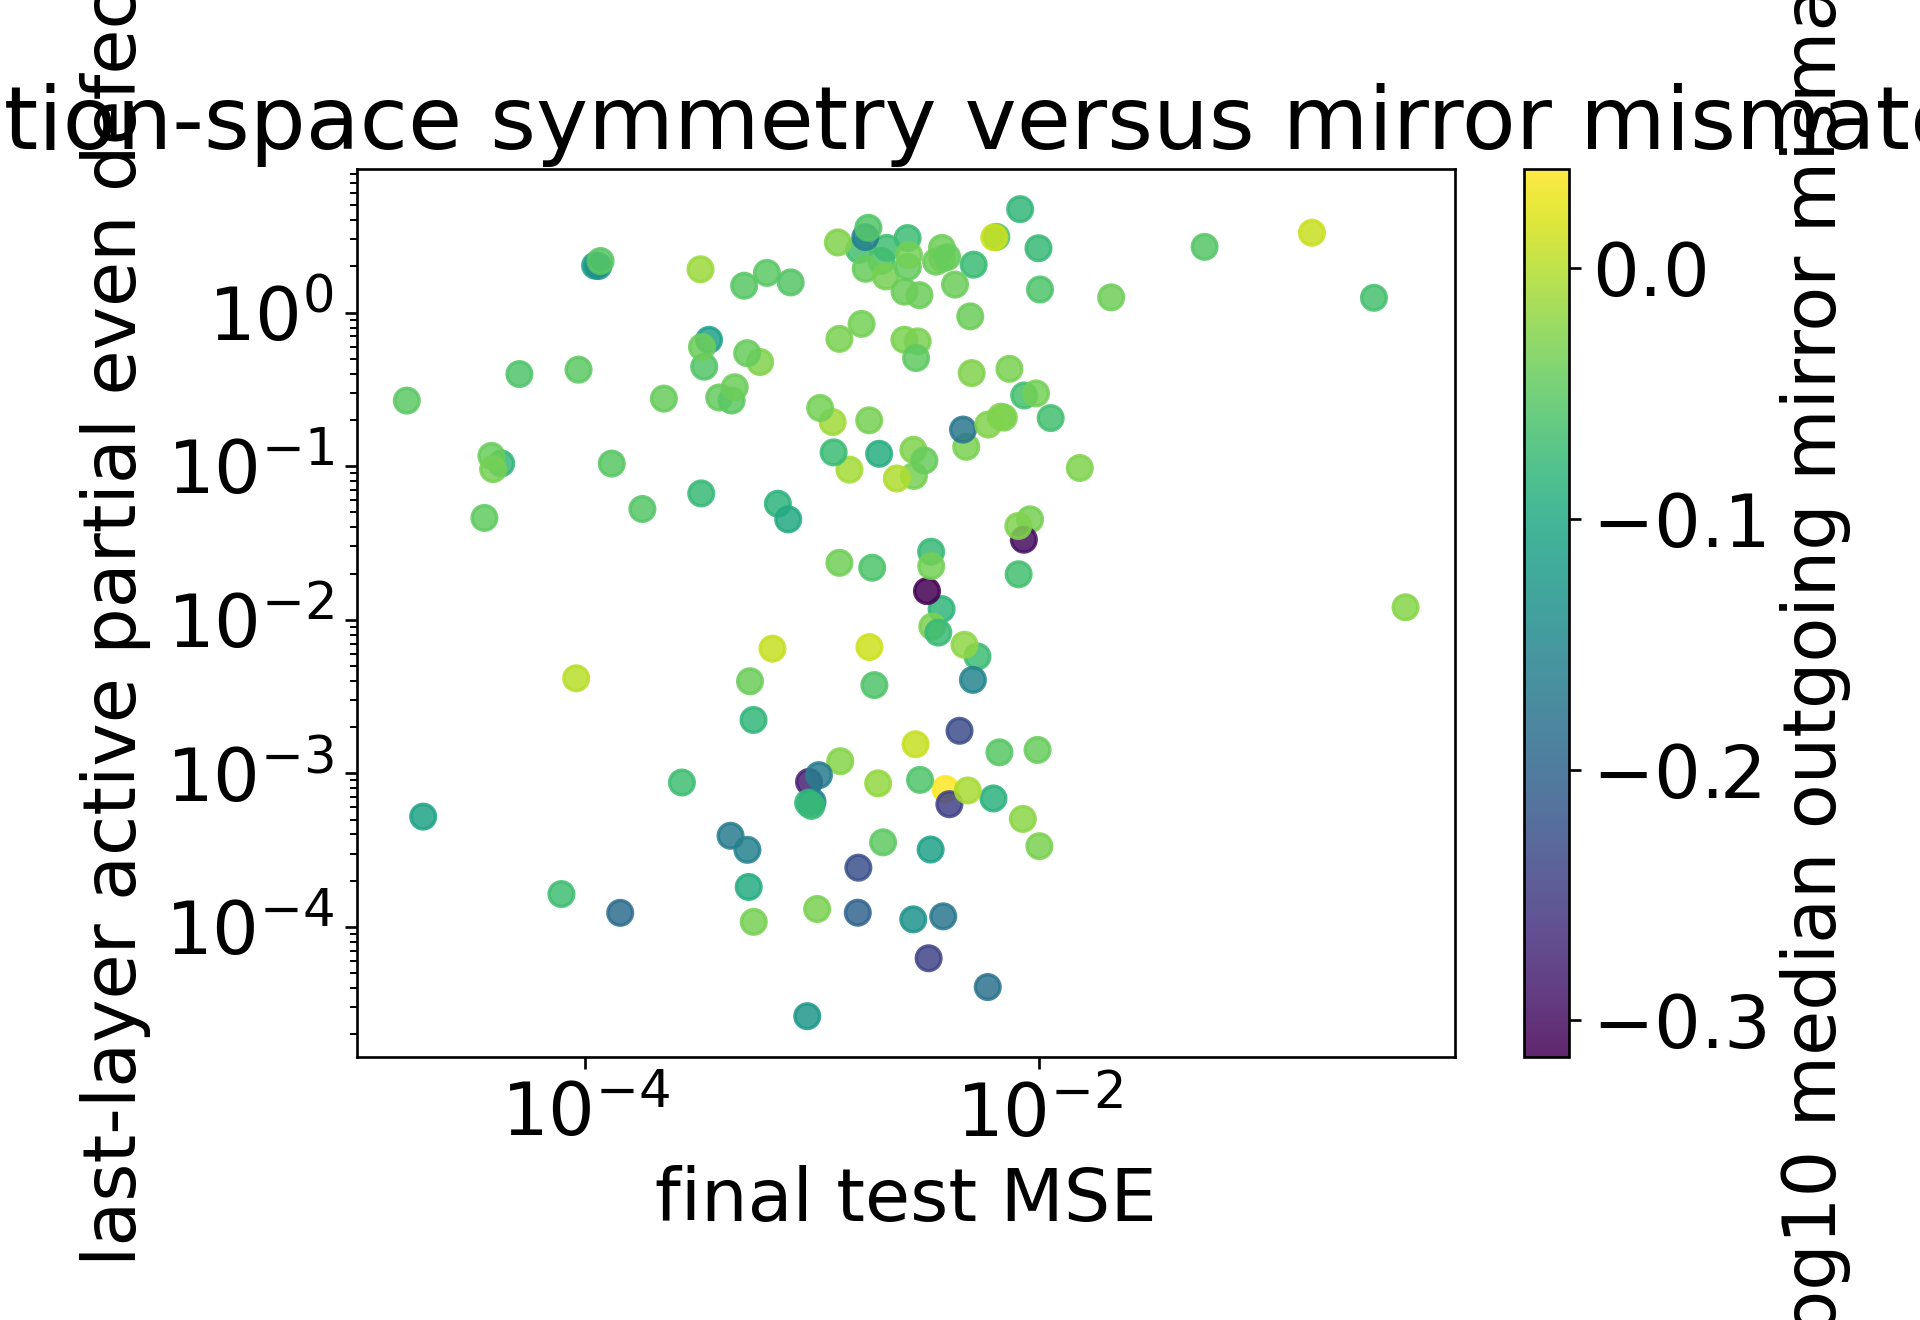
\includegraphics[width=0.72\linewidth]{results/weightspace_distributions/loss_partial_vs_mirror_mismatch.png}
\caption{Completed ICLR reruns: final test MSE versus active partial symmetry, colored by median outgoing mirror mismatch in weight space.}
\end{figure}

\begin{figure}[h]
\centering
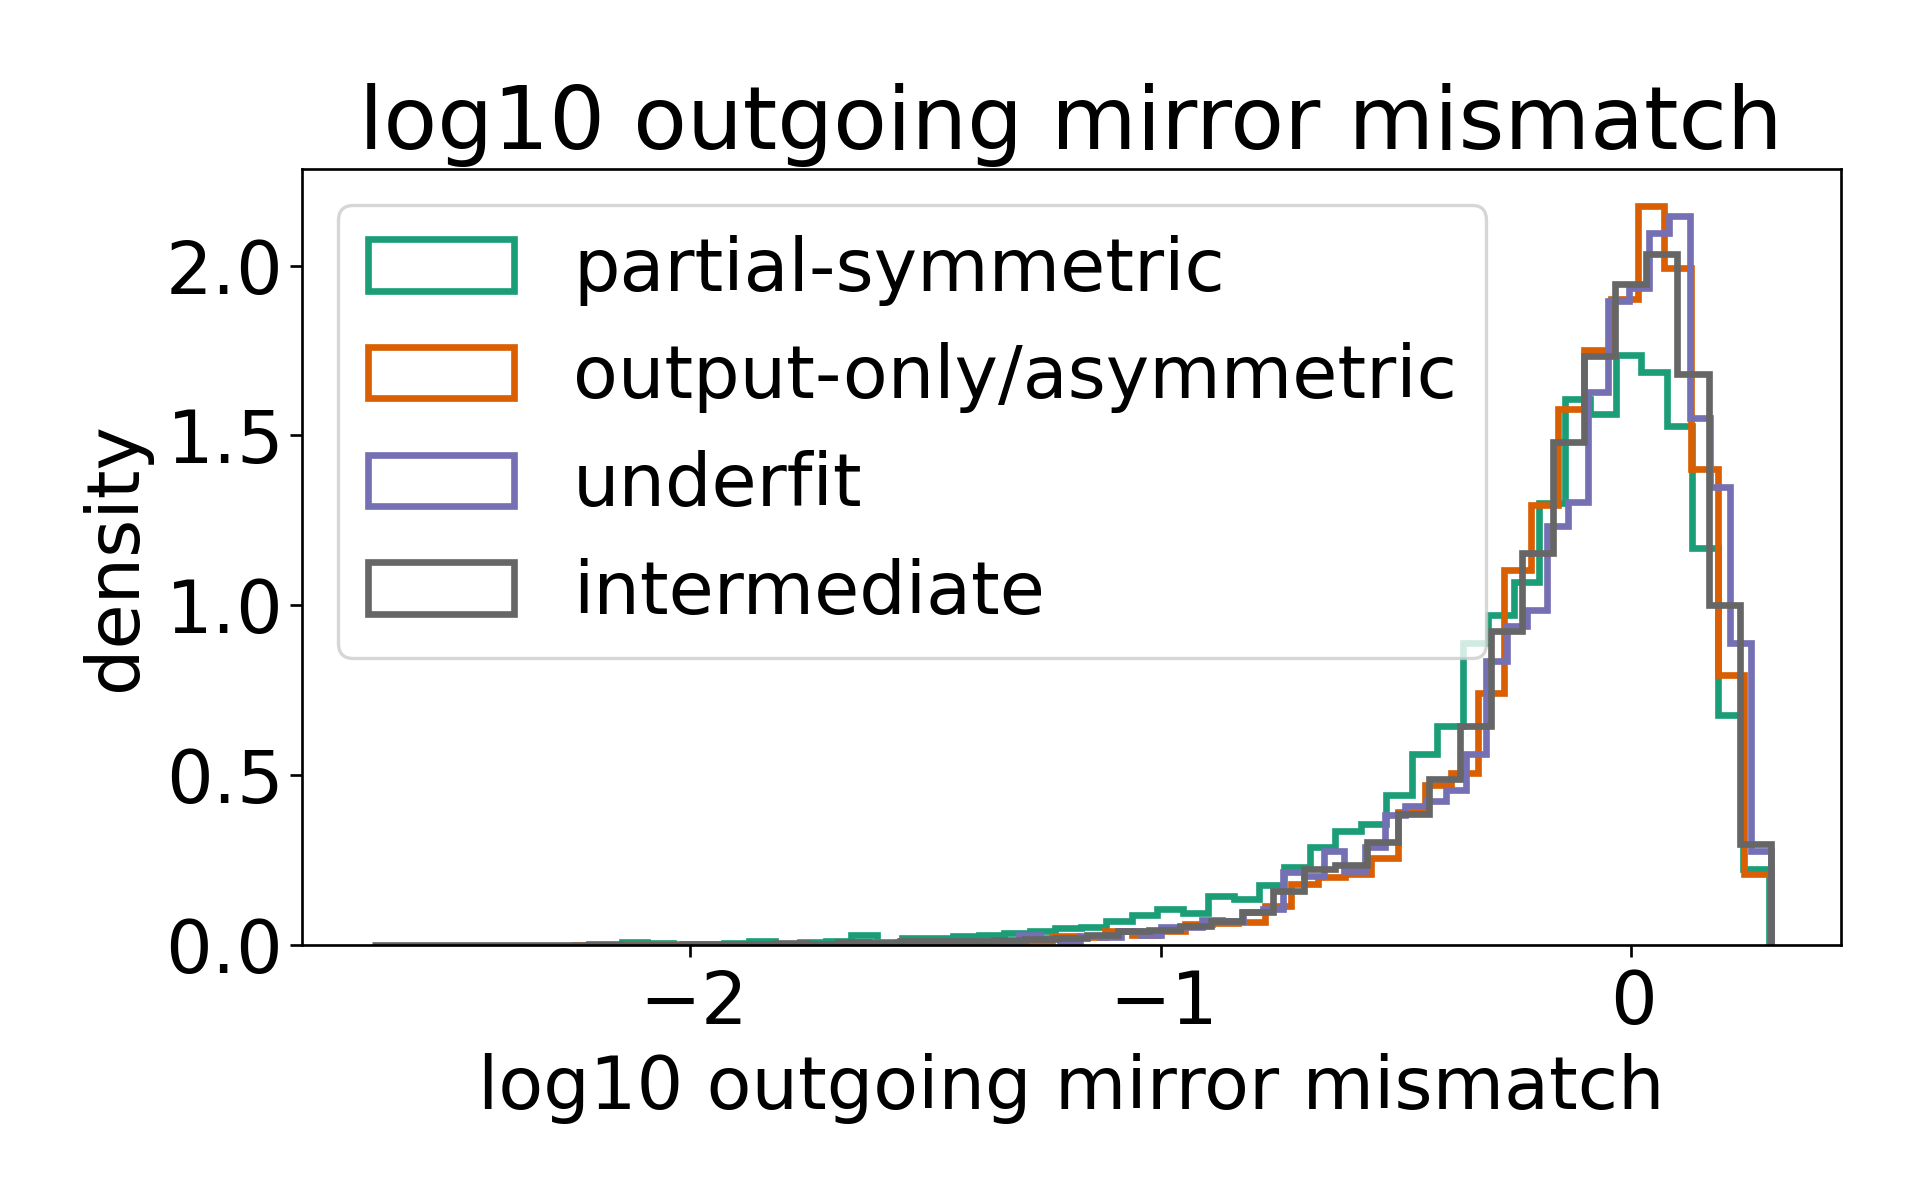
\includegraphics[width=0.72\linewidth]{results/weightspace_distributions/outgoing_mismatch_distribution.png}
\caption{Distribution of outgoing mirror-pair mismatch across partial-symmetric, output-only/asymmetric, intermediate, and underfit regimes.}
\end{figure}

\begin{figure}[h]
\centering
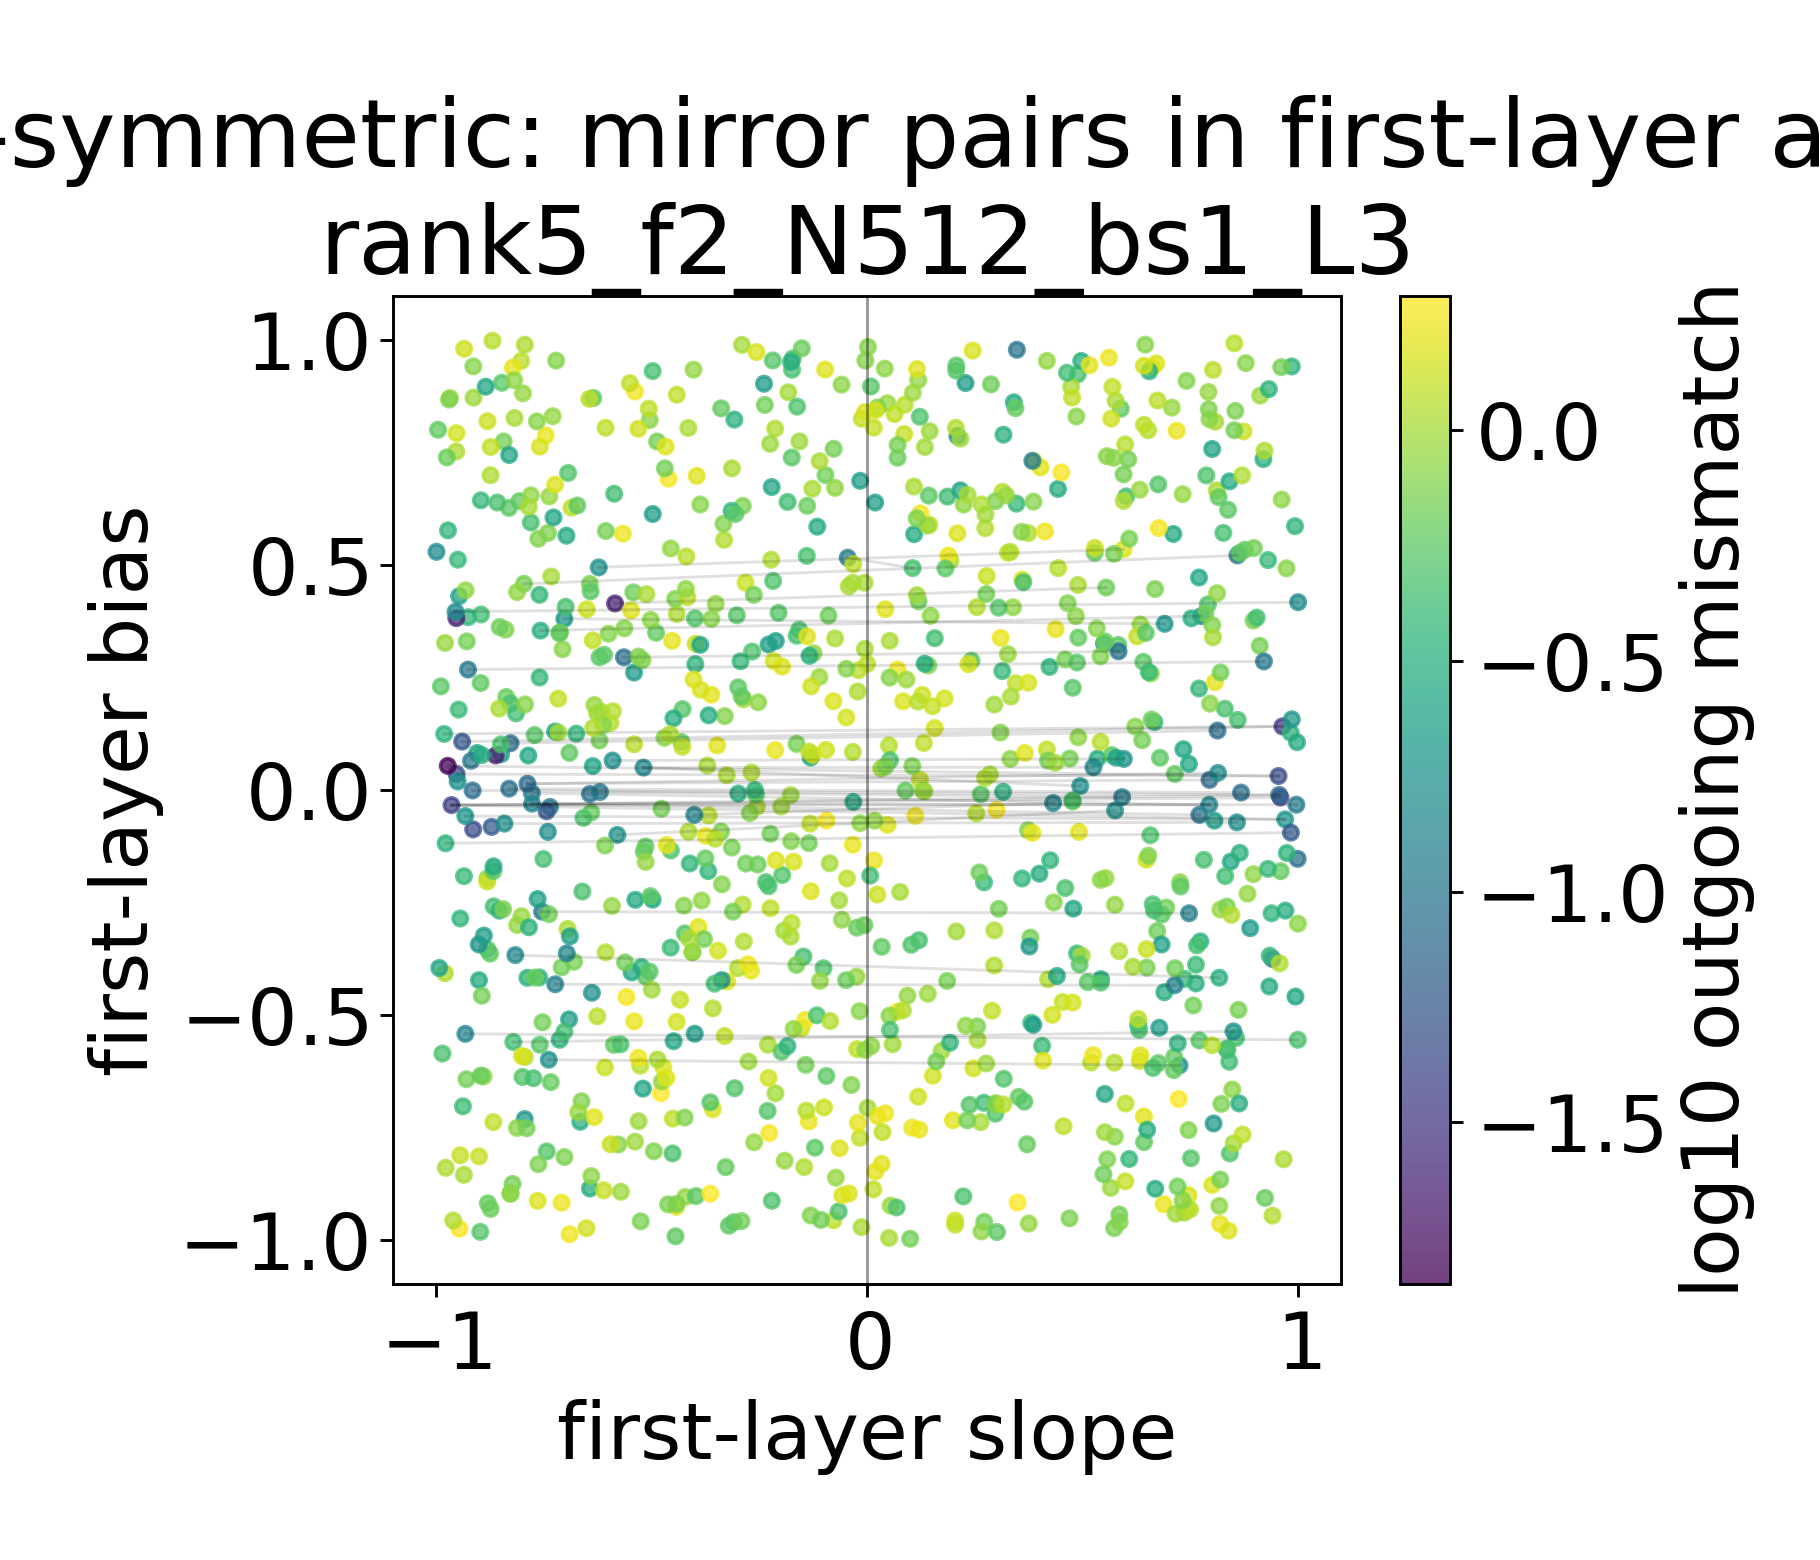
\includegraphics[width=0.48\linewidth]{results/weightspace_distributions/example_partial-symmetric_mirror_pairs.png}
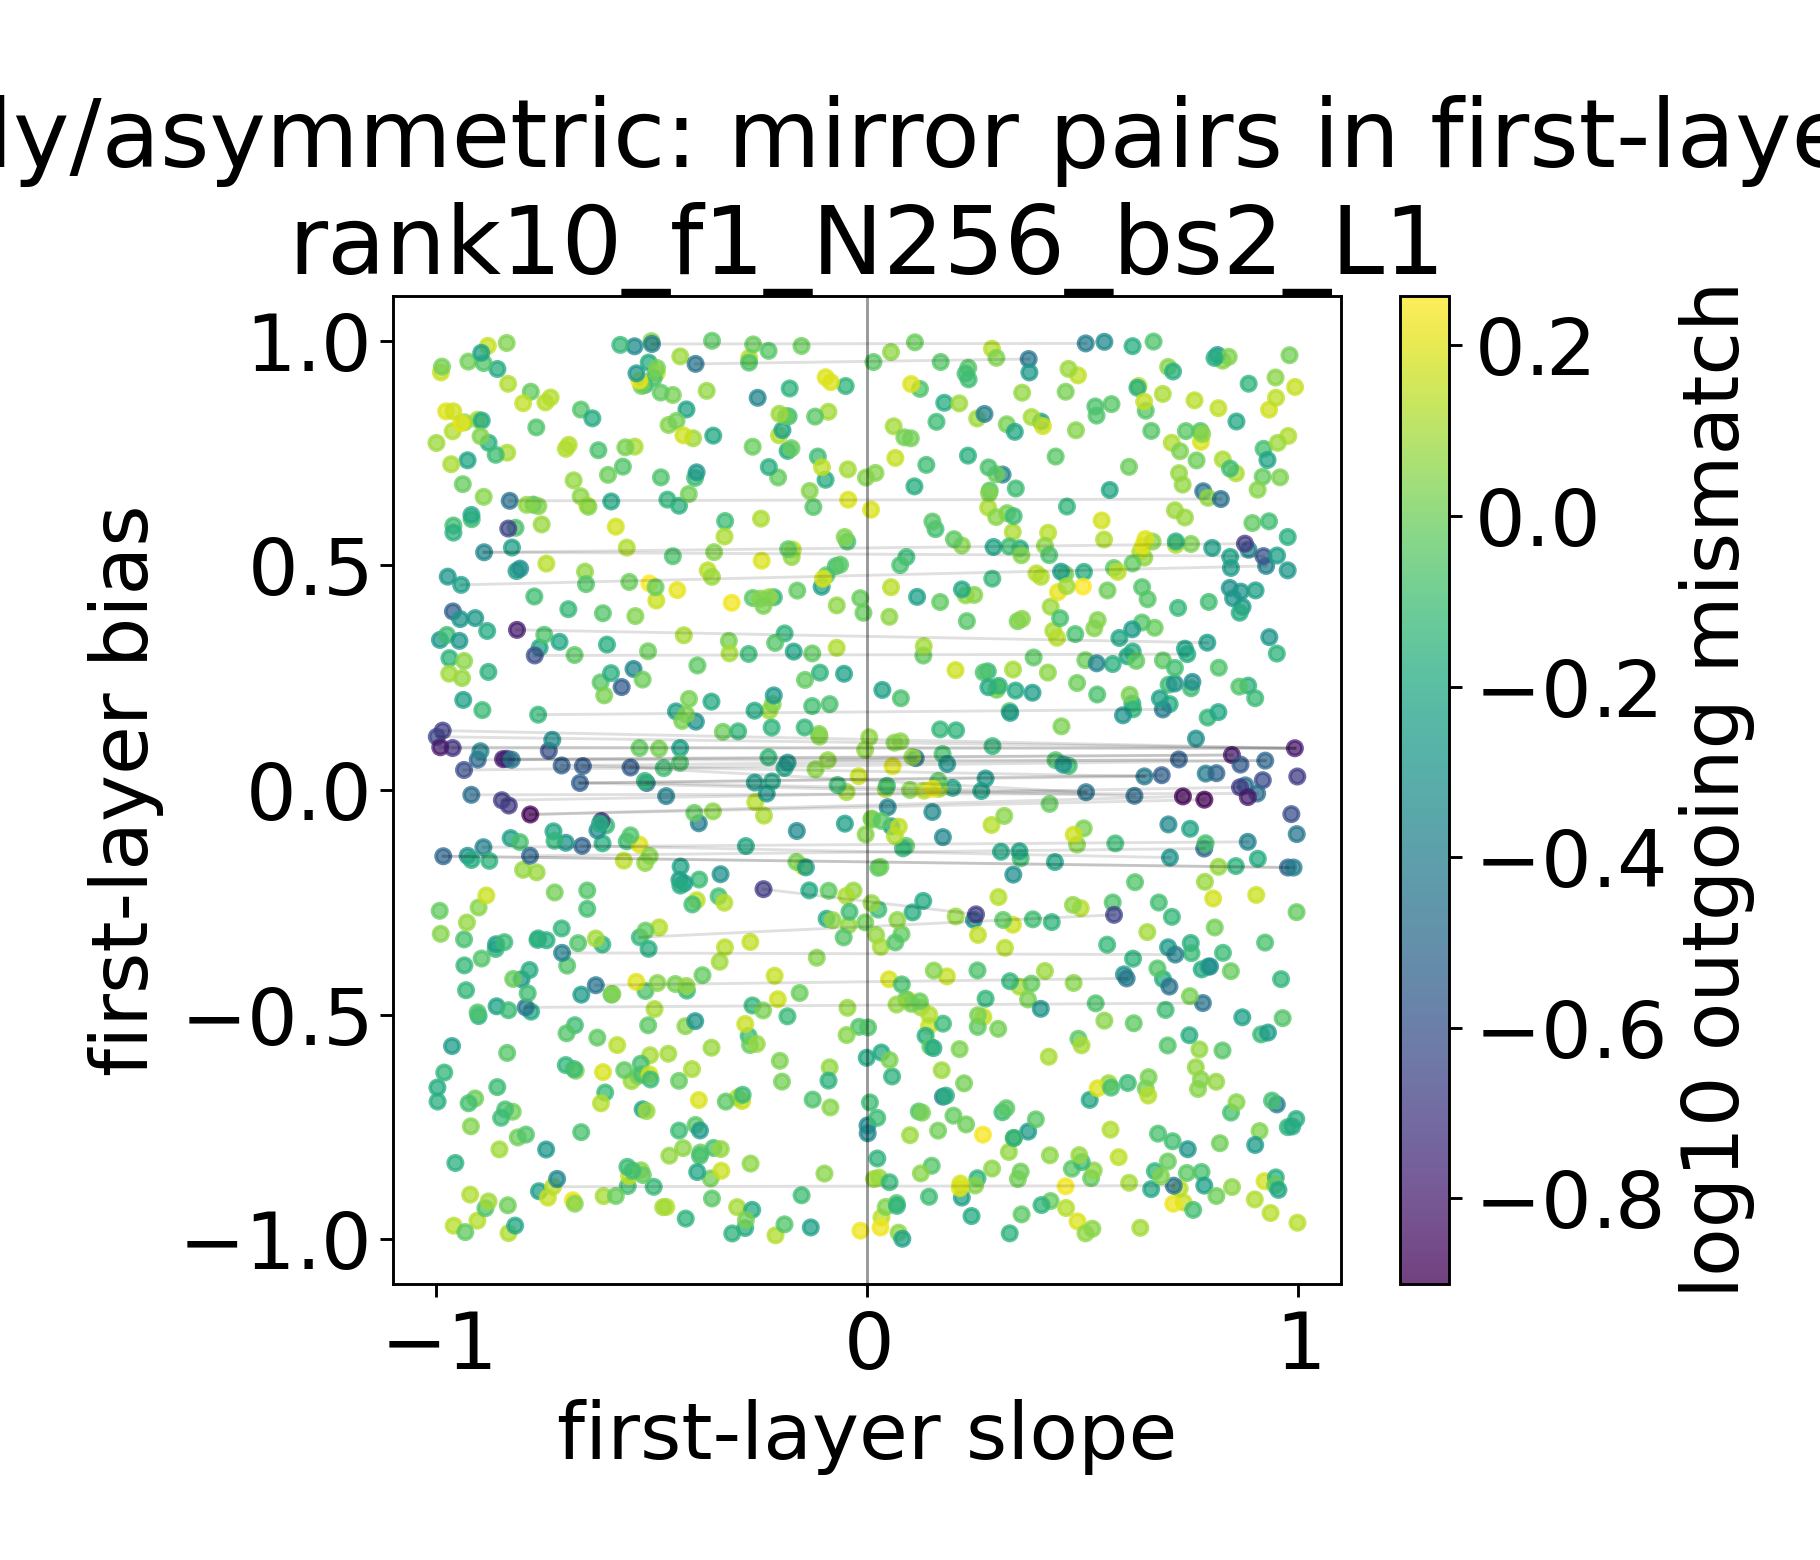
\includegraphics[width=0.48\linewidth]{results/weightspace_distributions/example_output-only_asymmetric_mirror_pairs.png}
\caption{First-layer atoms $(a_j,b_j)$ and nearest mirror-pair links for a symmetric run (left) and an output-only/asymmetric run (right). Color denotes outgoing coefficient mismatch.}
\end{figure}

\section{MNIST Batch-Size Ablation}

We also include a practical MNIST ablation to test whether the same optimizer and representation diagnostics are meaningful beyond controlled even targets. We train a width-$128$, depth-$2$ MLP and MMNNs with ranks $10$ and $25$ on a 2000-sample MNIST subset for 20 epochs with SGD. Batch size ranges from $1$ to full batch. Since MNIST labels are not invariant under arbitrary flips or shifts, the reported transform defects are representation-stability proxies rather than direct symmetry claims.

The main effect is batch size. Small-batch SGD learns; large-batch and full-batch training stall, especially for MMNN. For example, the MLP reaches $90.3\%$ test accuracy at batch $1$ and $64.2\%$ at full batch. MMNN rank $10$ reaches $83.9\%$ at batch $1$ but only $10.5\%$ at full batch. Thus MNIST supports the landscape/optimization side of the story: stochasticity is important for entering useful representation regimes, and symmetry metrics must be interpreted together with task performance.

Because the large-batch SGD losses are not low enough, we reran the failing regimes with Adam. Adam substantially improves the MLP and partially rescues MMNN at batch $512$: MLP batch $512$ improves from $84.3\%$ to $89.0\%$, and MMNN rank $25$ batch $512$ improves from $29.7\%$ to $67.1\%$. Full-batch MMNN remains poor after 20 epochs, improving only from $19.7\%$ to $33.0\%$ at rank $25$. Thus low loss is essential before interpreting any symmetry metric: undertrained full-batch MMNN can look stable only because its logits are weak.

\begin{figure}[h]
\centering
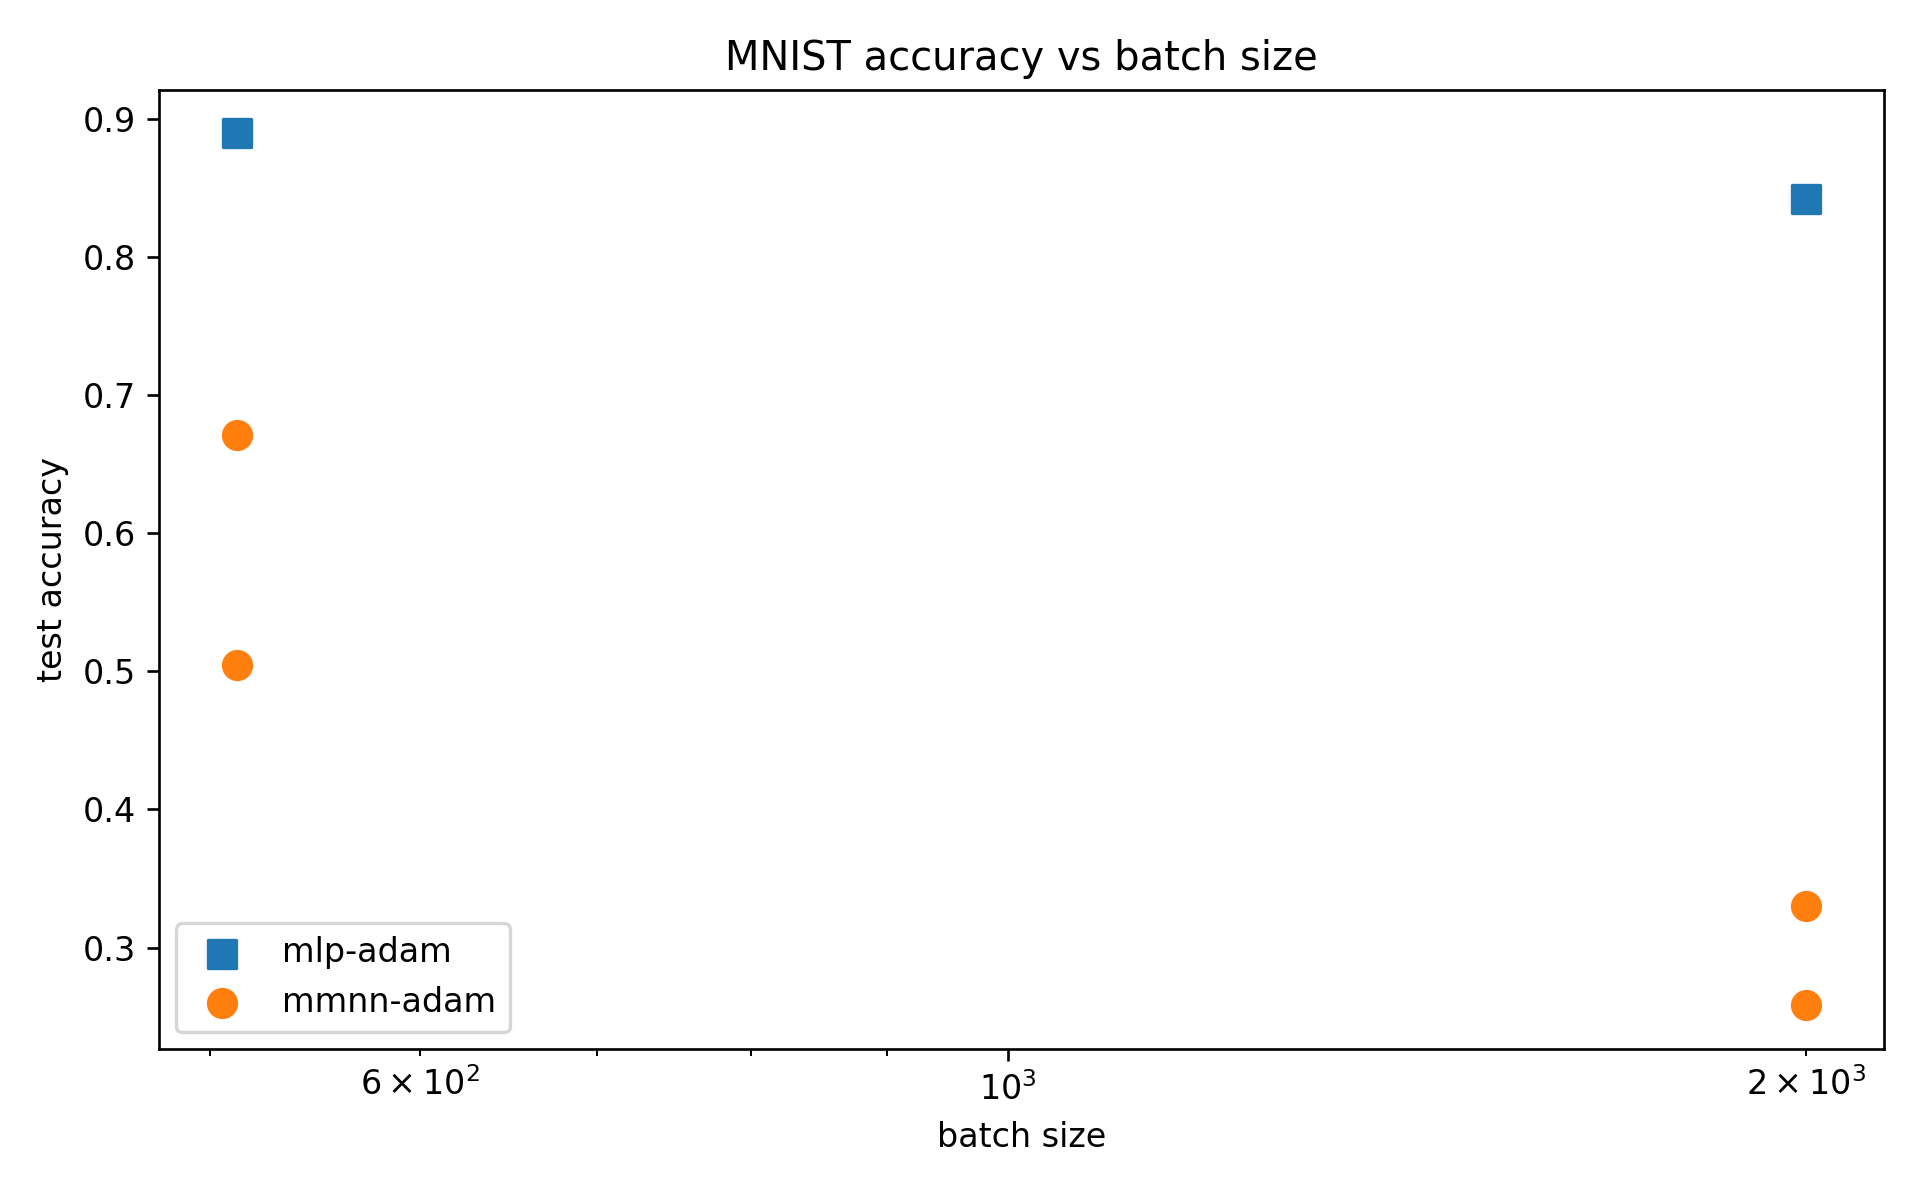
\includegraphics[width=0.72\linewidth]{results/mnist_batch_symmetry/mnist_accuracy_vs_batch.png}
\caption{MNIST practical ablation: test accuracy versus batch size for MLP and MMNN.}
\end{figure}

\begin{figure}[h]
\centering
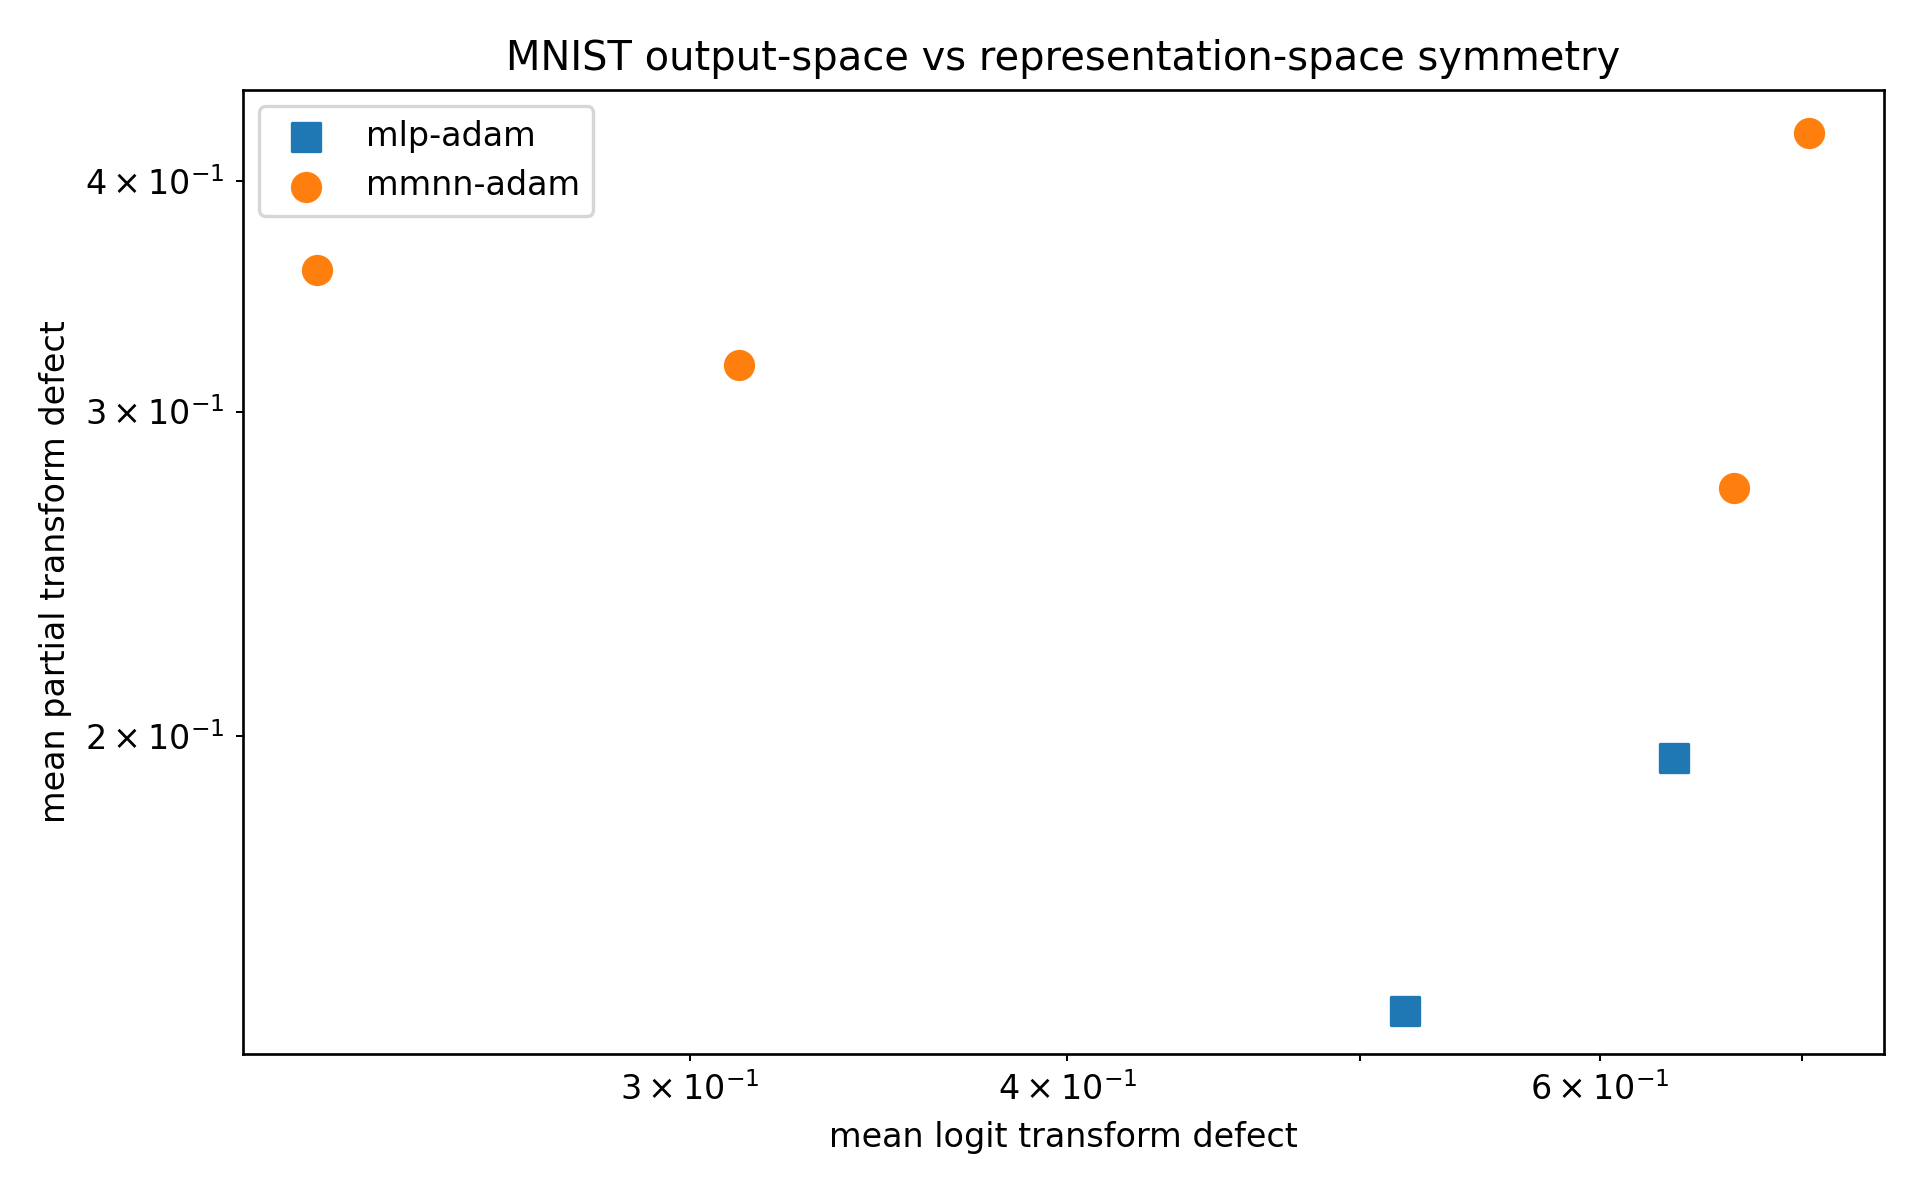
\includegraphics[width=0.72\linewidth]{results/mnist_batch_symmetry/mnist_output_vs_partial_defect.png}
\caption{MNIST transform-defect diagnostics. These are representation-stability proxies, not label-preserving symmetry guarantees.}
\end{figure}

\begin{figure}[h]
\centering
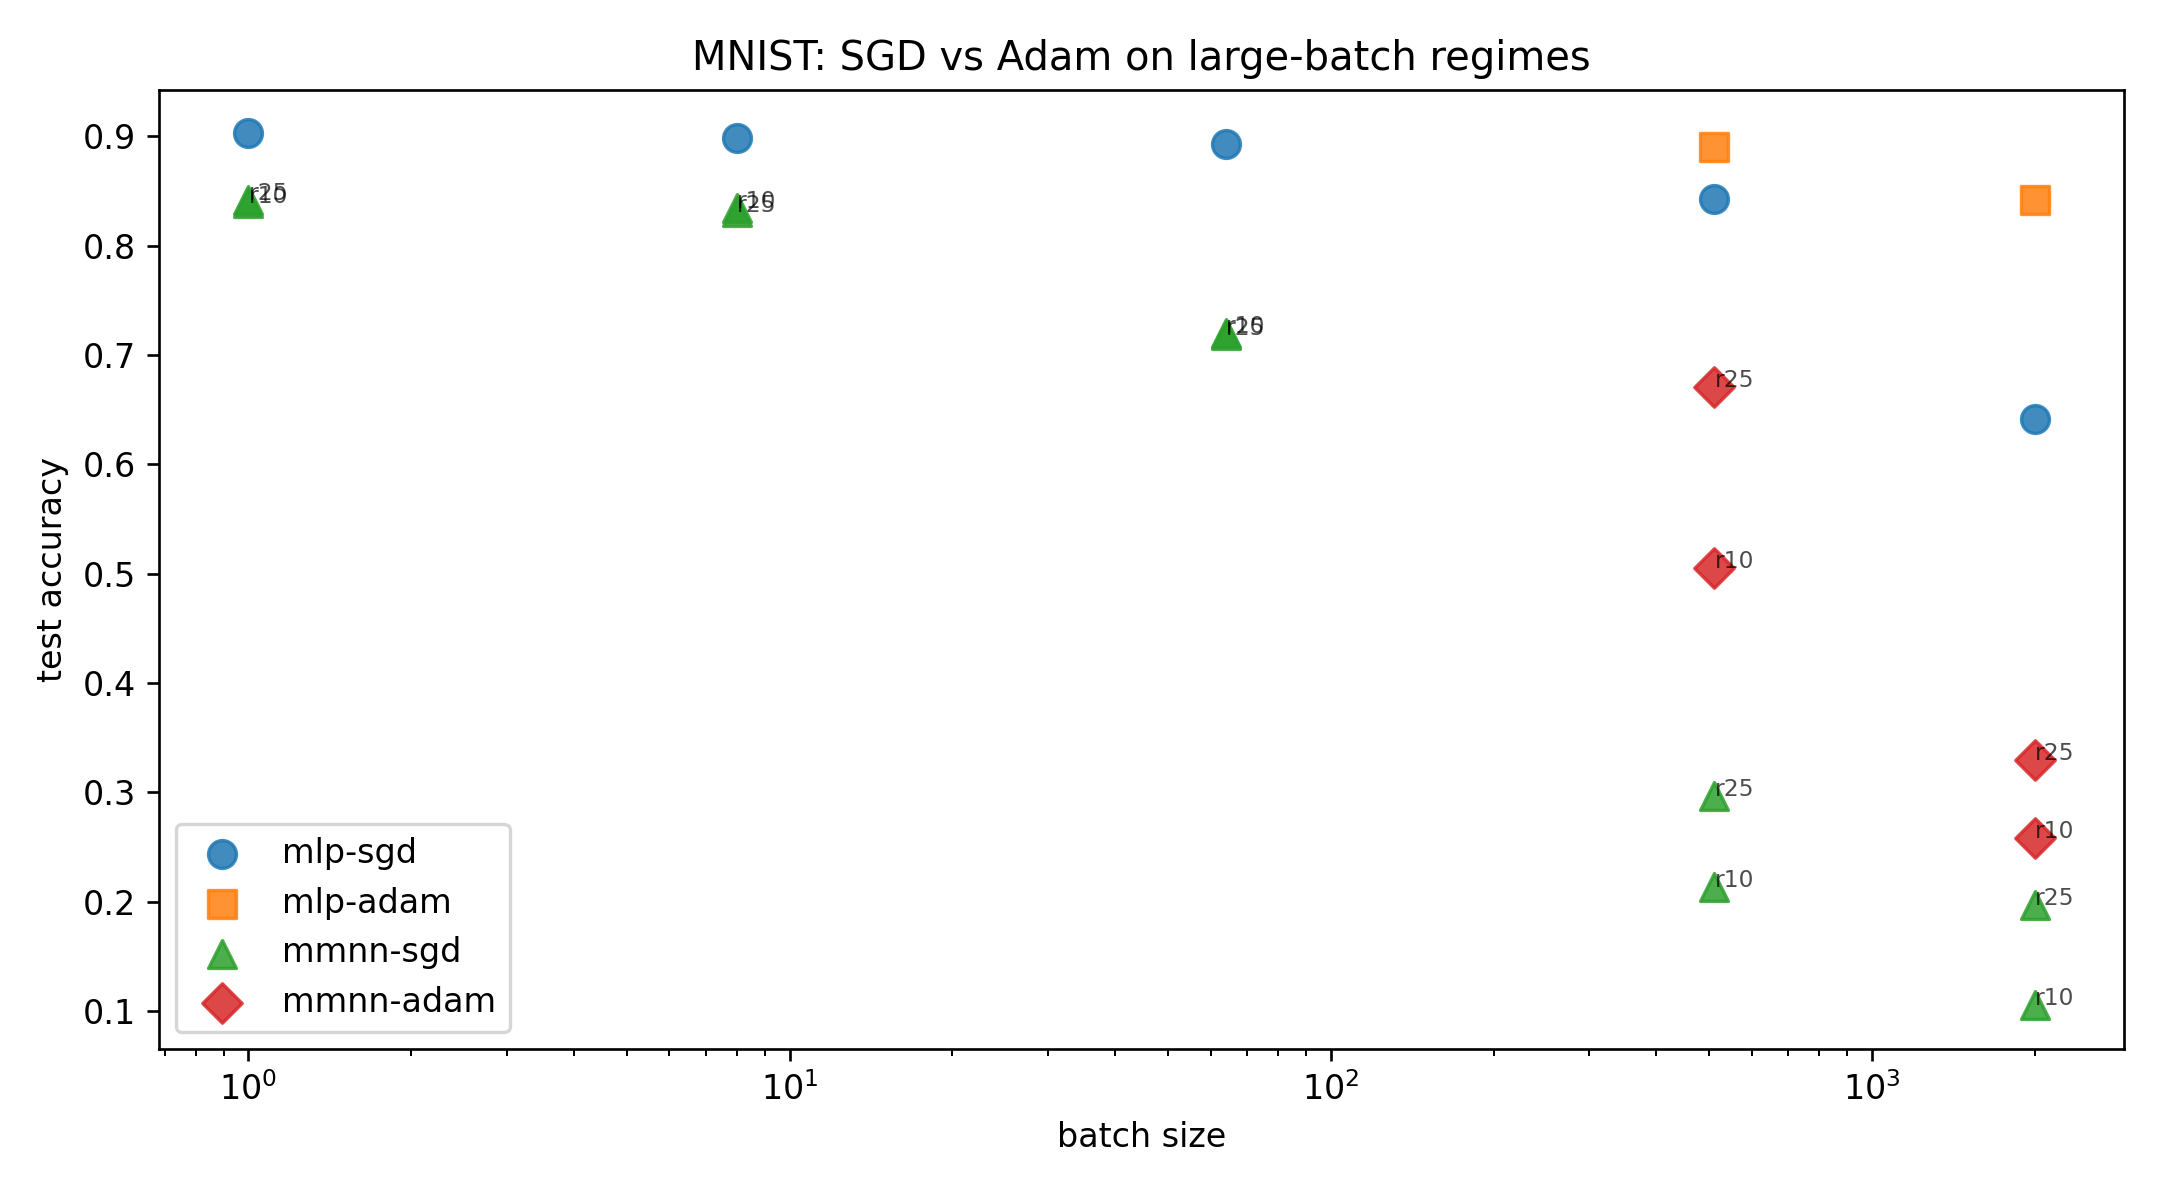
\includegraphics[width=0.72\linewidth]{results/mnist_batch_symmetry/optimizer_accuracy_vs_batch.png}
\caption{MNIST optimizer follow-up on large-batch regimes. Adam rescues MLP and partly improves MMNN at batch $512$, but full-batch MMNN still fails in this short run.}
\end{figure}

\begin{figure}[h]
\centering
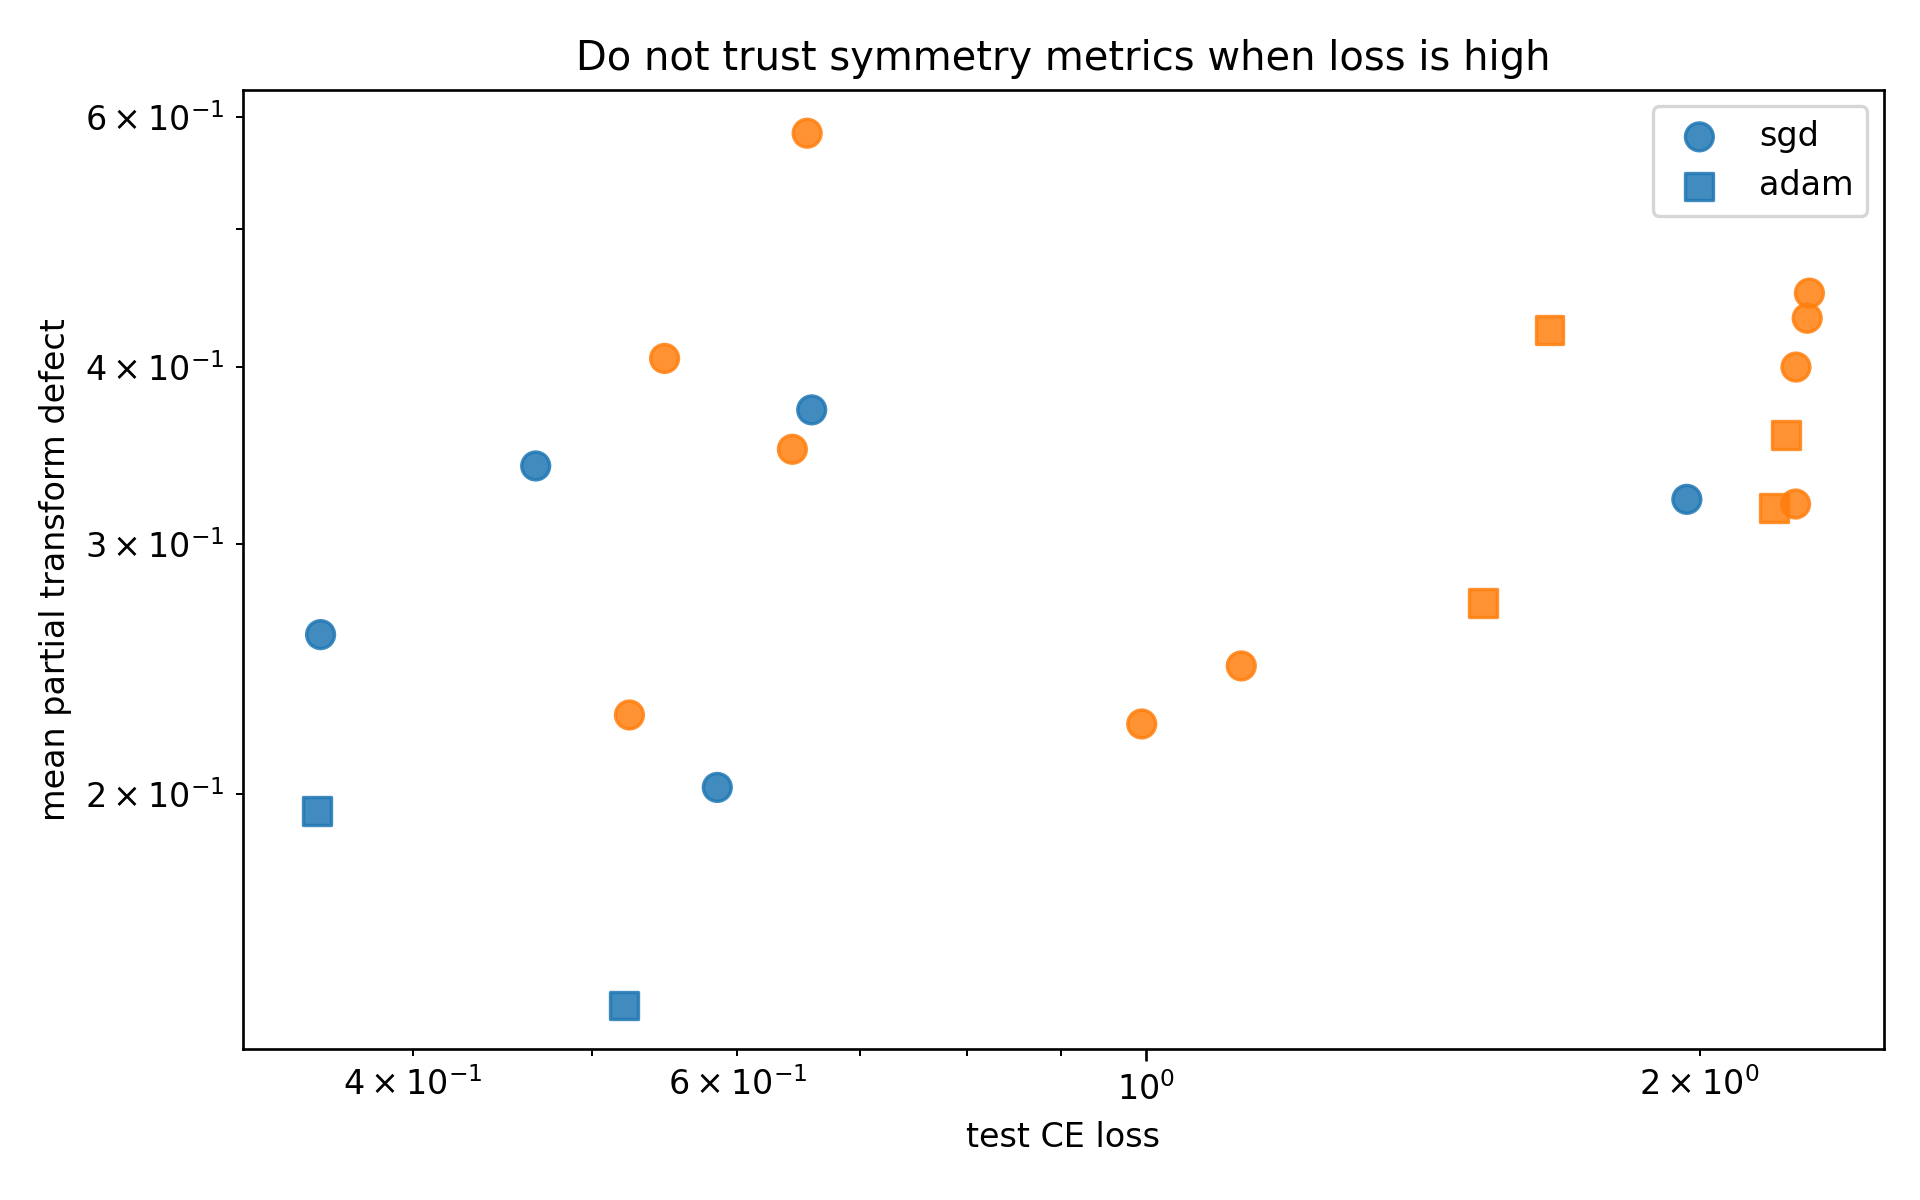
\includegraphics[width=0.72\linewidth]{results/mnist_batch_symmetry/optimizer_loss_vs_partial_defect.png}
\caption{Symmetry diagnostics must be read together with loss: high-loss runs can have misleadingly small transform defects.}
\end{figure}

\section{Planned Claim}

The planned claim is not merely that the output is symmetric. The stronger claim is that low-rank networks learn symmetric partial functions and that this is visible as organized mirror structure in the trained weights. Full-rank networks may fit the same even target while using asymmetric hidden features, which suggests symmetry breaking inside landscape valleys.

\end{document}
